\chapter{Design}
% Indicating the structure of the system, with particular focus on main ideas of the design, unusual design features, etc.
% Describe the design of your program. Justify the decisions you made.
%%%%%%%%%%%%%%%%%%%%%%%%%%%%%%%%%%%%%%%\section{JUSTIFY DECISIONS!!!!!!!!!!}
\section{Level Generation}
\subsection{Contextualising the Wave Function Collapse Algorithm}
The \acrfull{wfc} algorithm can be viewed as an extension on the ideas presented by the \acrfull{mac3} algorithm. What is referred to as a grid of cells with tile choices in \acrlong{wfc} is analogous to a graph of variables / nodes with a domain of possible values. Constraints between variables can then be viewed as edges in an undirected graph (Figure \ref{fig:undirectedGraph}).

% Diagram of a directed graph

\begin{figure}[H]
    \centering
    \subfigure[Undirected graph]{
        \begin{tikzpicture}[circlenode/.style={circle, draw=black, very thick, minimum size=5mm}]
            %Nodes
            \node[circlenode]      (00)                              {0,0};
            \node[circlenode]      (01)       [right=of 00]          {0,1};
            \node[circlenode]      (02)       [right=of 01]          {0,2};
            \node[circlenode]      (10)       [above=of 00]          {1,0};
            \node[circlenode]      (11)       [right=of 10]          {1,1};
            \node[circlenode]      (12)       [right=of 11]          {1,2};
            \node[circlenode]      (20)       [above=of 10]          {2,0};
            \node[circlenode]      (21)       [right=of 20]          {2,1};
            \node[circlenode]      (22)       [right=of 21]          {2,2};

            %Lines
            \draw[-] (00.north) -- (10.south);
            \draw[-] (10.north) -- (20.south);
            \draw[-] (01.north) -- (11.south);
            \draw[-] (11.north) -- (21.south);
            \draw[-] (02.north) -- (12.south);
            \draw[-] (12.north) -- (22.south);

            \draw[-] (00.east) -- (01.west);
            \draw[-] (01.east) -- (02.west);
            \draw[-] (10.east) -- (11.west);
            \draw[-] (11.east) -- (12.west);
            \draw[-] (20.east) -- (21.west);
            \draw[-] (21.east) -- (22.west);
        \end{tikzpicture}
        \label{fig:undirectedGraph}
    }
    \hfill
    \subfigure[Directed graph]{
        \begin{tikzpicture}[circlenode/.style={circle, draw=black, very thick, minimum size=5mm}]
            %Nodes
            \node[circlenode]      (00)                              {0,0};
            \node[circlenode]      (01)       [right=of 00]          {0,1};
            \node[circlenode]      (02)       [right=of 01]          {0,2};
            \node[circlenode]      (10)       [above=of 00]          {1,0};
            \node[circlenode]      (11)       [right=of 10]          {1,1};
            \node[circlenode]      (12)       [right=of 11]          {1,2};
            \node[circlenode]      (20)       [above=of 10]          {2,0};
            \node[circlenode]      (21)       [right=of 20]          {2,1};
            \node[circlenode]      (22)       [right=of 21]          {2,2};

            %Lines

            \draw[->] (00.800) -- (10.280);
            \draw[->] (10.800) -- (20.280);
            \draw[->] (01.800) -- (11.280);
            \draw[->] (11.800) -- (21.280);
            \draw[->] (02.800) -- (12.280);
            \draw[->] (12.800) -- (22.280);

            \draw[<-] (00.100) -- (10.260);
            \draw[<-] (10.100) -- (20.260);
            \draw[<-] (01.100) -- (11.260);
            \draw[<-] (11.100) -- (21.260);
            \draw[<-] (02.100) -- (12.260);
            \draw[<-] (12.100) -- (22.260);

            \draw[->] (00.350) -- (01.190);
            \draw[->] (01.350) -- (02.190);
            \draw[->] (10.350) -- (11.190);
            \draw[->] (11.350) -- (12.190);
            \draw[->] (20.350) -- (21.190);
            \draw[->] (21.350) -- (22.190);

            \draw[<-] (00.370) -- (01.170);
            \draw[<-] (01.370) -- (02.170);
            \draw[<-] (10.370) -- (11.170);
            \draw[<-] (11.370) -- (12.170);
            \draw[<-] (20.370) -- (21.170);
            \draw[<-] (21.370) -- (22.170);
        \end{tikzpicture}
        \label{fig:directedGraph}
    }

    \caption{A \(3\times3\) cell grid as an undirected and directed graph}
    \label{fig:graphs}
\end{figure}

\subsection{Arcs}
An edge in an undirected graph can alternatively be viewed as two opposite edges in a directed graph (Figure \ref{fig:directedGraph}). Arcs apply this concept to constraints, with each arc representing one of the two edges making up a constraint in the directed graph. For an arc to be locally arc consistent, all the values in the first variable's domain must be supported by at least one value in the second variable's domain.

For example, suppose the use of an extremely simple tile set with only cubes and empty tiles, where any tile choice is possible at the start. Furthermore, say that cubes can only have other cubes as neighbours and that empty tiles only have empty tiles as neighbours. This corresponds to Figure \ref{fig:arcsStart}.

\begin{figure}[H]
    \centering
    \begin{tikzpicture}[circlenode/.style={circle, draw=black, very thick, minimum size=5mm}]
        %Nodes
        \node[circlenode, label={[align=center]\{Cube, Empty\}}]      (00)                                            {A};
        \node[circlenode, label={[align=center]\{Cube, Empty\}}]      (01)       [right=of 00, xshift=1.5cm]          {B};
        \node[circlenode, label={[align=center]\{Cube, Empty\}}]      (02)       [right=of 01, xshift=1.5cm]          {C};

        %Lines
        \draw[->] (00.350) -- (01.190);
        \draw[<-] (00.370) -- (01.170);
        \draw[->] (01.350) -- (02.190);
        \draw[<-] (01.370) -- (02.170);
    \end{tikzpicture}
    \caption{Example starting state, in which all arcs are consistent}
    \label{fig:arcsStart}
\end{figure}

Then, assume that node A is set to be a cube, removing the empty tile from its domain. Now, the arc <A,B> is consistent as B still has a cube as a support value. However, the arc <B,A> is no longer consistent since the empty tile does not have any support in A's domain, which only has the cube in it. This corresponds to Figure \ref{fig:arcsAssigned}.

% Diagram showing two arcs of a constraint
\begin{figure}[H]
    \centering
    \begin{tikzpicture}[circlenode/.style={circle, draw=black, very thick, minimum size=5mm}]
        %Nodes
        \node[circlenode, label={[align=center]\{Cube\}}]      (00)                                            {A};
        \node[circlenode, label={[align=center]\{Cube, Empty\}}]      (01)       [right=of 00, xshift=1.5cm]          {B};
        \node[circlenode, label={[align=center]\{Cube, Empty\}}]      (02)       [right=of 01, xshift=1.5cm]          {C};

        %Lines
        \draw[->] (00.350) -- (01.190);
        \draw[<-, dashed] (00.370) -- (01.170);
        \draw[->] (01.350) -- (02.190);
        \draw[<-] (01.370) -- (02.170);
    \end{tikzpicture}
    \caption{After assigning Cube to A, <B,A> is no longer consistent}
    \label{fig:arcsAssigned}
\end{figure}

\subsection{AC3}
The \acrfull{ac3} algorithm enforces arc consistency in the grid of cells. The algorithm is given a queue of arcs to enforce arc consistency across. Each arc is checked for support and unsupported domain values pruned. If any domain changes occur, then all arcs targeting the primary variable of the current arc are re-added to the queue. This is required as the domain change may have resulted in support for arcs to this variable being lost.

% Diagram showing arc revision
Back to the example, assigning Cube to A will trigger arc revision with all the arcs incident on A. In this case, this initialises the queue with arc <B,A>. Checking the arc shows that B's Empty value is no longer supported by A (Figure \ref{fig:arcRevision}).

\begin{figure}[H]
    \begin{framed}
        \begin{enumerate}
            \item Check arc <B,A>:
                  \begin{enumerate}
                      \item B's value Cube has support in A through its value Cube.
                      \item B's value Empty does NOT have support in A! Remove it from the domain.
                  \end{enumerate}
        \end{enumerate}
    \end{framed}
    \caption{Revising arc <B,A>}
    \label{fig:arcRevision}
\end{figure}

Performing this single revision leaves the graph in the state as shown in Figure \ref{fig:arcsRevised1}. Revising <B,A> results in <C,B> becoming inconsistent, highlighting the importance of adding targeted arcs to the queue after a domain change. In this case, <C,B> must be added to the queue. <A,B> does not have to be added since the domain change happened while revising <B,A>. This exploits the fact that arc support is bi-directional, meaning that if a value is supported on <B,A>, then it must be supporting some value on arc <A,B>.

\begin{figure}[H]
    \centering
    \begin{tikzpicture}[circlenode/.style={circle, draw=black, very thick, minimum size=5mm}]
        %Nodes
        \node[circlenode, label={[align=center]\{Cube\}}]      (00)                                            {A};
        \node[circlenode, label={[align=center]\{Cube\}}]      (01)       [right=of 00, xshift=1.5cm]          {B};
        \node[circlenode, label={[align=center]\{Cube, Empty\}}]      (02)       [right=of 01, xshift=1.5cm]          {C};

        %Lines
        \draw[->] (00.350) -- (01.190);
        \draw[<-] (00.370) -- (01.170);
        \draw[->] (01.350) -- (02.190);
        \draw[<-,dashed] (01.370) -- (02.170);
    \end{tikzpicture}

    \caption{Revising <B,A> results in <C,B> becoming inconsistent}
    \label{fig:arcsRevised1}
\end{figure}

Revision of <C,B> proceeds similarly to revision of <B,A> (Figure \ref{fig:arcRevision}). Similarly, C's domain change from revision of <C,B> does not require re-checking of arc <B,C>. After this, the queue of arcs to revise is empty and as such the consistency before assignment has been maintained. The state after revision is shown in Figure \ref{fig:arcsRevised2}.

\begin{figure}[H]
    \centering
    \begin{tikzpicture}[circlenode/.style={circle, draw=black, very thick, minimum size=5mm}]
        %Nodes
        \node[circlenode, label={[align=center]\{Cube\}}]      (00)                                            {A};
        \node[circlenode, label={[align=center]\{Cube\}}]      (01)       [right=of 00, xshift=1.5cm]          {B};
        \node[circlenode, label={[align=center]\{Cube\}}]      (02)       [right=of 01, xshift=1.5cm]          {C};

        %Lines
        \draw[->] (00.350) -- (01.190);
        \draw[<-] (00.370) -- (01.170);
        \draw[->] (01.350) -- (02.190);
        \draw[<-] (01.370) -- (02.170);
    \end{tikzpicture}

    \caption{The graph after \acrshort{ac3} has been carried out}
    \label{fig:arcsRevised2}
\end{figure}

An additional property to note is that each node now only has one value in its domain. Given that each arc is consistent, this means that this is a valid solution to the original problem where each node could either be a cube or empty tile. In the context of \acrshort{wfc}, this means that all cells have been collapsed with a valid tile choice and thus that a valid map has been generated.

\subsection{MAC3}
\acrfull{mac3} uses \acrfull{ac3} to create a full constraint solving algorithm. To begin, \acrshort{ac3} is run with all arcs to ensure global arc consistency at the start. Then, a variable and value are chosen in an attempt to find a solution. This choice is like that done in the example shown previously in Figure \ref{fig:arcsAssigned}. Arc consistency is then maintained by running \acrshort{ac3} with the all the arcs targeting the variable that had a value assigned (Figure \ref{fig:arcRevision}). This ensures that these arcs maintain local arc consistency. As global arc consistency was enforced at the start, maintaining local arc consistency after each assignment is enough to also maintain global arc consistency. If any variable assignments lead to a domain wipeout (an empty domain) when enforcing arc consistency, then backtracking can be performed and another value chosen. Once each variable only has one value left and all arcs are consistent, a solution has been found. If not stopped by a timeout, \acrshort{mac3} will continue running until a solution has been found or all choices have been attempted, meaning that there is no solution.

\subsection{Playing Sudoku as an Analogue to Constraint Solving}
Sudoku can serve as an example to make the constraint solving process clearer. Someone solving Sudoku might pencil in the possible number for each cell to help make guesses and fill the grid. This is analogous to giving each cell a set of possible values.

At the start, given numbers help the player pencil each remaining cell. Like this, the possible numbers of each cell are reduced. If a cell only has one possible number remaining, then the player knows that the cell must hold that value. This is analogous to running \acrshort{ac3} at the start to ensure each cell has a consistent set of possible values.

Eventually, the player is likely to face the situation where no more numbers can be inferred from the given clues. Just like the \acrshort{mac3} solver, the player must make a guess as to what the correct number might be. After making a guess, the implications of it can be carried forward. This is analogous to running \acrshort{ac3} after making a variable assignment.

If this guess was incorrect and leads to a cell with no choices remaining, the player must undo the guess. This is analogous to having a domain wipeout and backtracking. After backtracking, the player knows that the choice they made was incorrect, so can pencil out the number they tried. From this, they may gain more clues about other cells in the grid. This is analogous to unassigning a value and running \acrshort{ac3} again.

If the player keeps making guesses and inferring additional information from them, they will eventually solve the Sudoku. If the player were to ignore the implications of a guess, then their solution may not be valid. This highlights the need to maintain consistency between each pair of constrained cells in the grid.

\subsection{Variable and Value Choice}\label{sec:variableAndValueChoice}
The manner in which a variable and value are chosen can be implemented as desired. The most effective method often depends on the specific problem. A common method used in \acrlong{wfc} is lowest entropy cell selection together with weighted random tile selection.

\subsubsection{Lowest Entropy Cell Selection}
The lowest entropy method can be viewed as choosing the most constrained cell at each step as it takes into account the weight of each cell. This increases the chance to find a solution quickly as any contradictory assignments are reached faster and backtracked from with fewer steps. The weight of each tile is defined in the level editor and represents the target rate of occurrence of a tile in the generated level. Equation \ref{shannonEntropy} shows the Shannon Entropy of a cell, which is lowest for cells with a small number of remaining tile choices of imbalanced weighting.% An example of this concept is shown in figure \ref{fig:entropyExample}.

% https://robertheaton.com/2018/12/17/wavefunction-collapse-algorithm/ - At latest 26.02.2024, but definitely before then.
\begin{align}
    \label{shannonEntropy}
    \text{Shannon Entropy}=S=\log(\sum{\text{weight}}) - \frac{\sum\left(\text{weight} \times \log(\text{weight})\right)}{\sum{\text{weight}}}
\end{align}

Figure \ref{fig:cellSelection} shows outputs of three different cell selection techniques. The lowest entropy cell selection generates a distinctly different level to the other two techniques. The two empty tile types have relative high weights. Furthermore, empty light tiles may only have empty tiles as neighbours. This means tiles near empty tiles will have a relatively low entropy, making them chosen before other tiles. In effect, this creates bigger clusters of empty space compared to the other selection techniques.%Furthermore, it was found that smallest domain cell selection resulted in longer solve times than the other two methods. This is likely due to 

\begin{figure}[H]
    \centering
    \subfigure[Ascending Cell Selection]{
        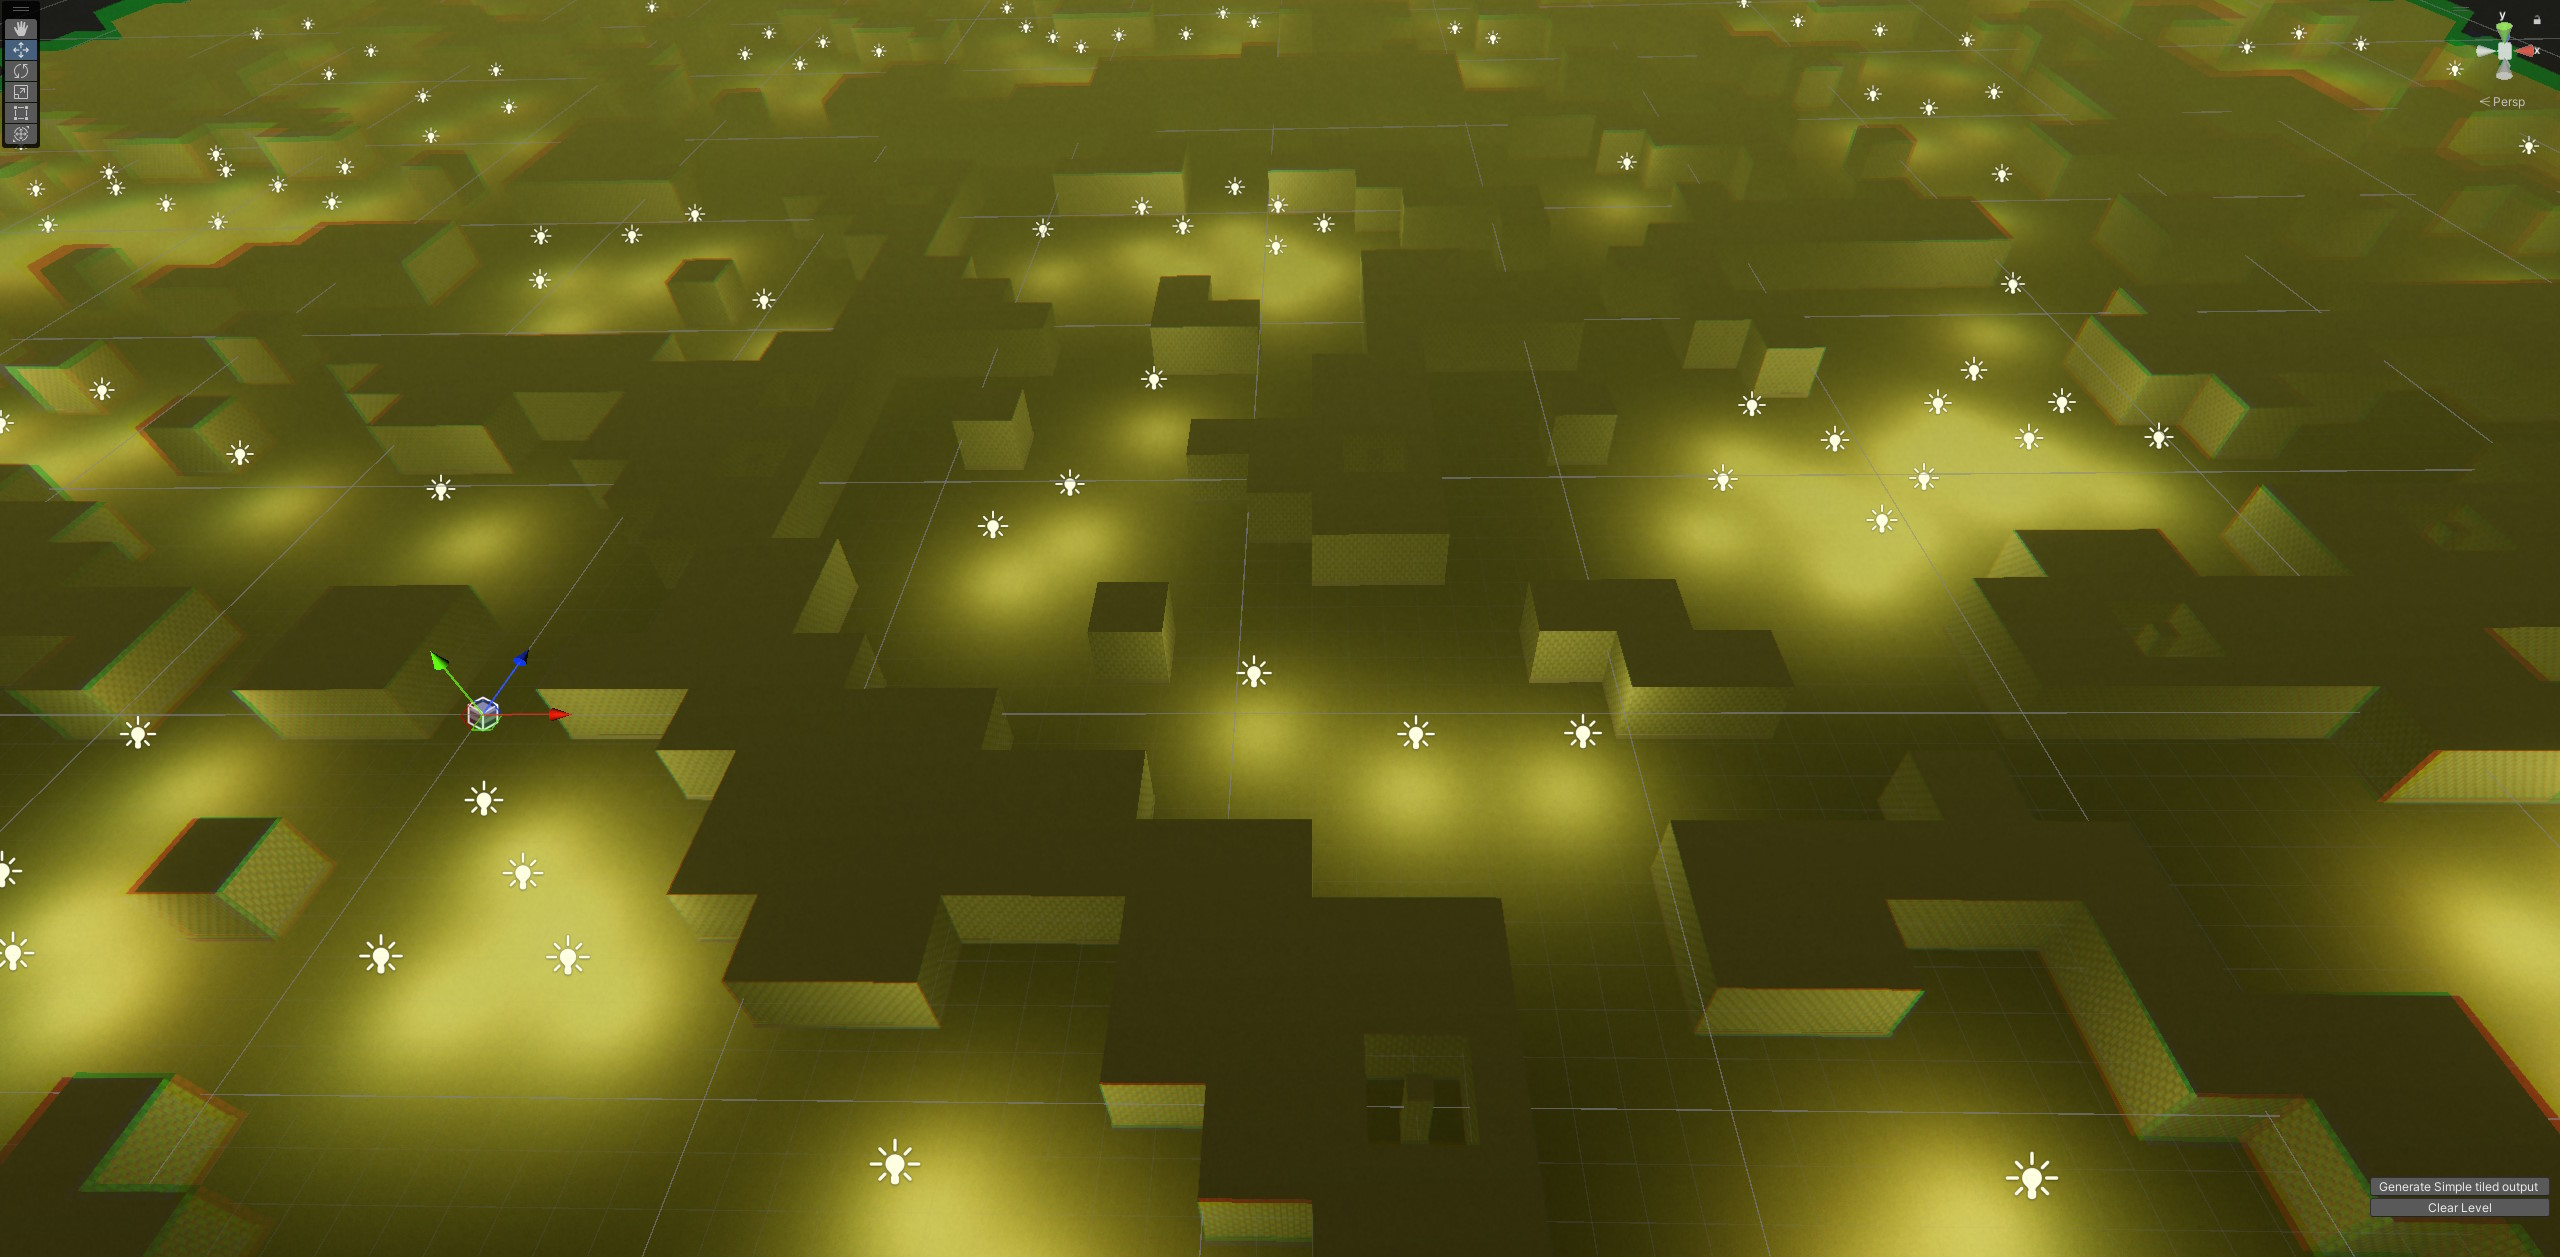
\includegraphics[width=0.475\textwidth, height=0.3\textheight, keepaspectratio]{Images/CellSelectionAscending.jpg}
        \label{fig:cellSelection1}
    }
    \hfill
    \subfigure[Smallest Domain Cell Selection]{
        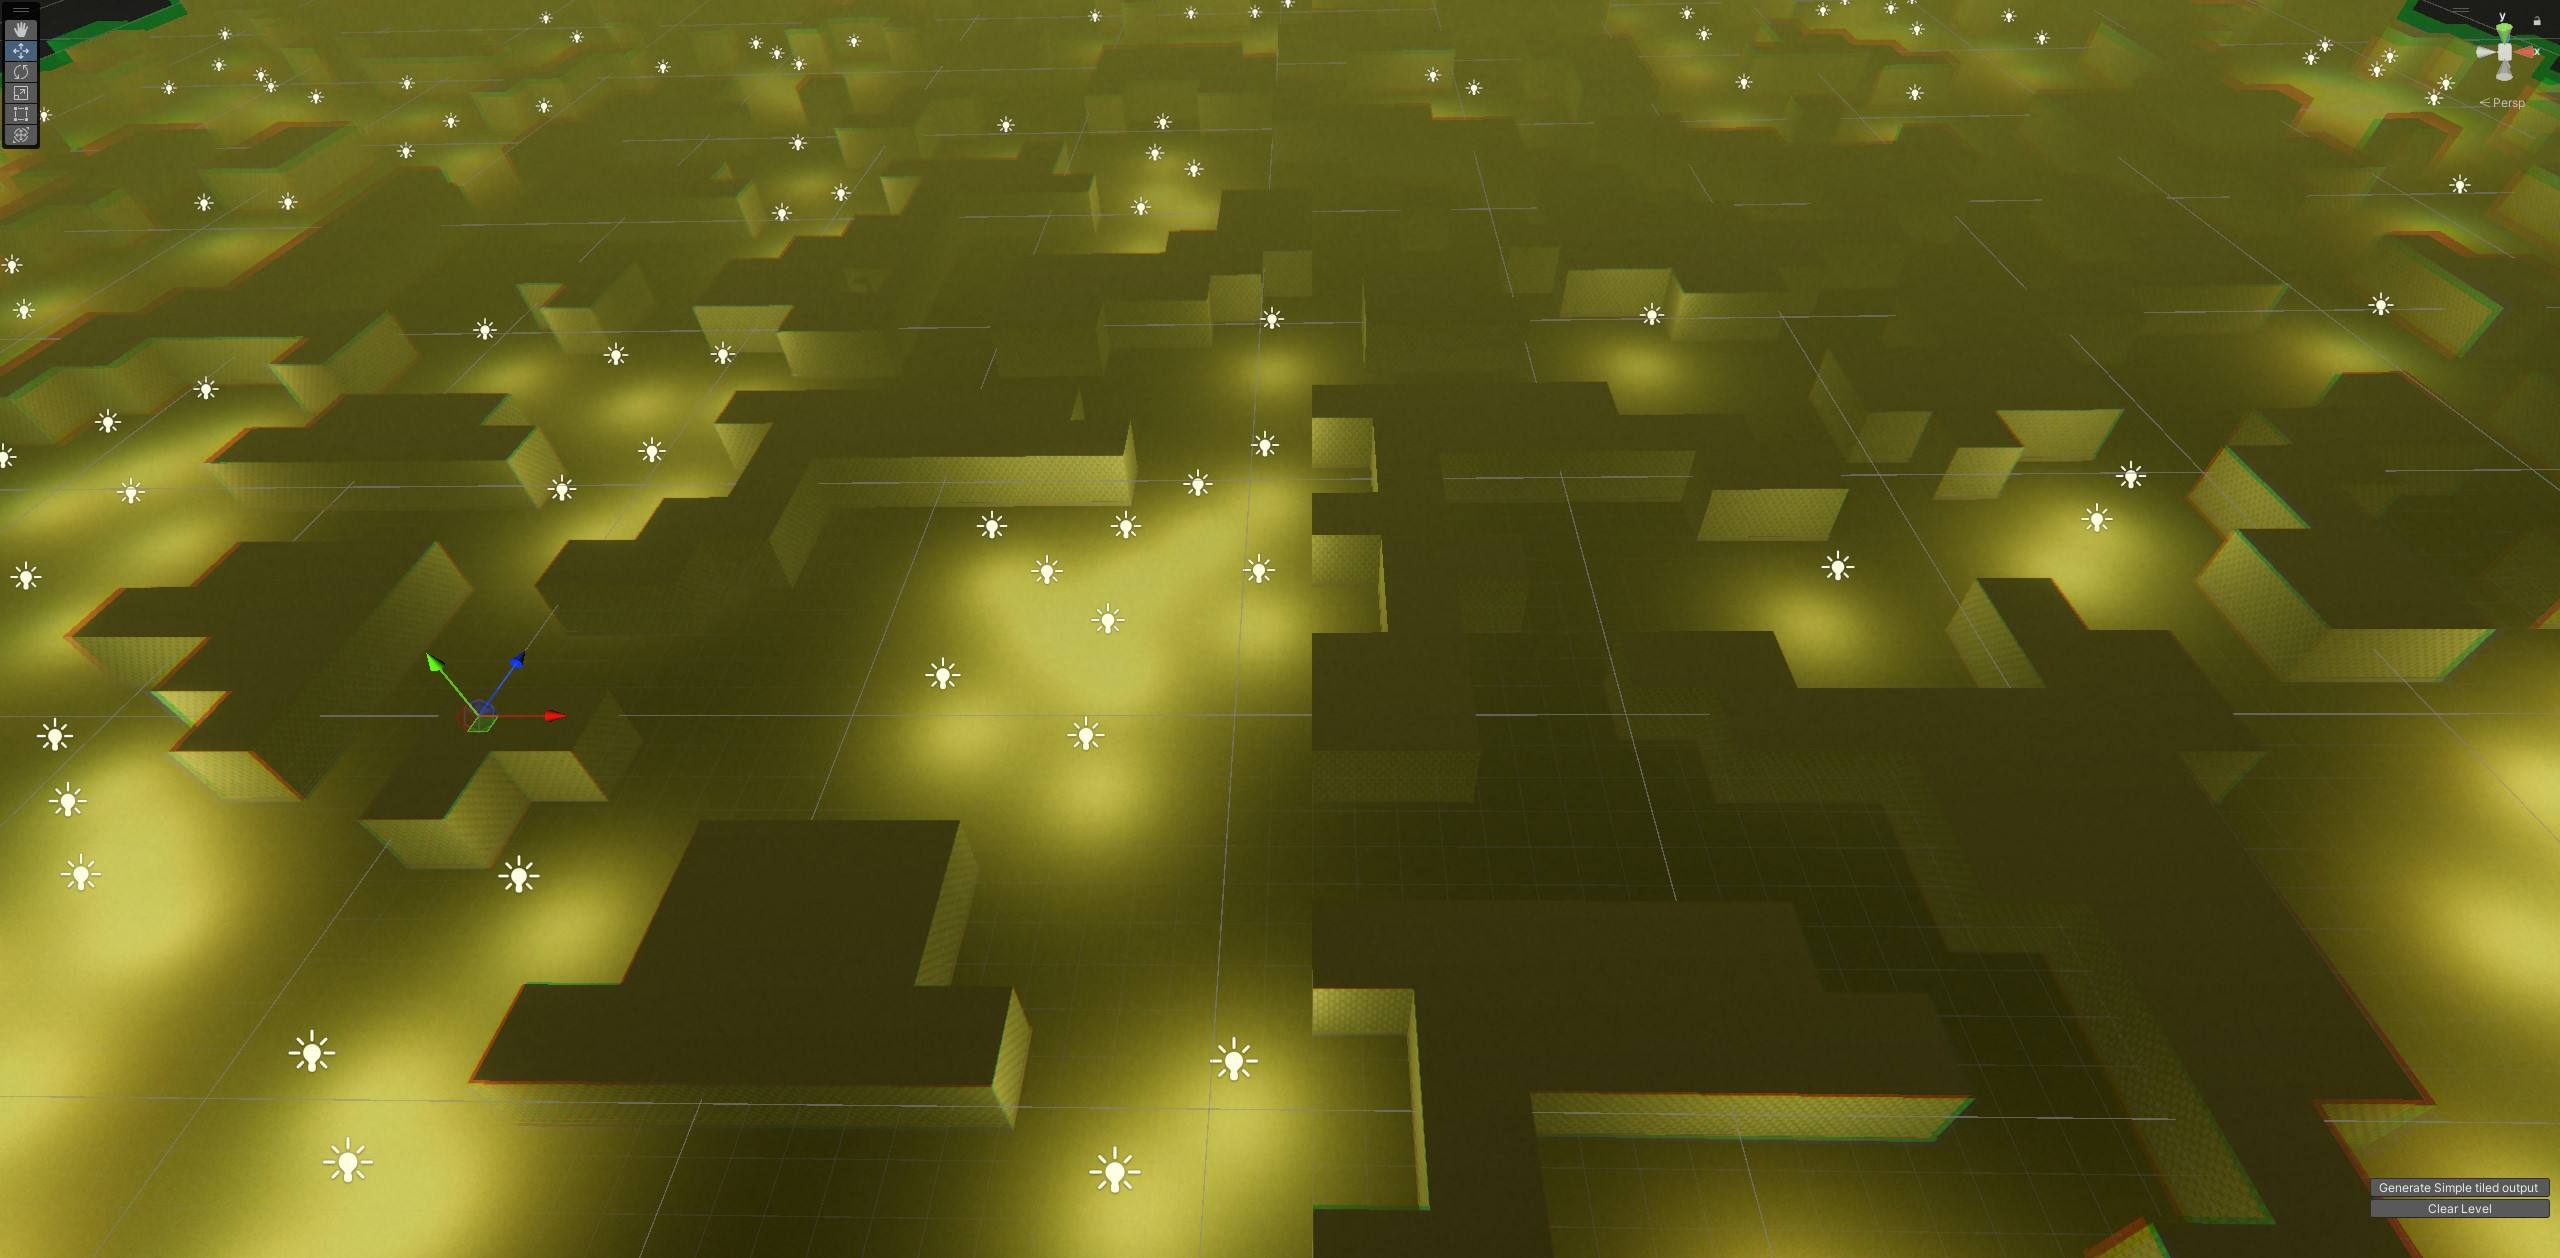
\includegraphics[width=0.475\textwidth, height=0.3\textheight, keepaspectratio]{Images/CellSelectionSmallestDomain.jpg}
        \label{fig:cellSelection2}
    }

    \subfigure[Lowest Entropy Cell Selection]{
        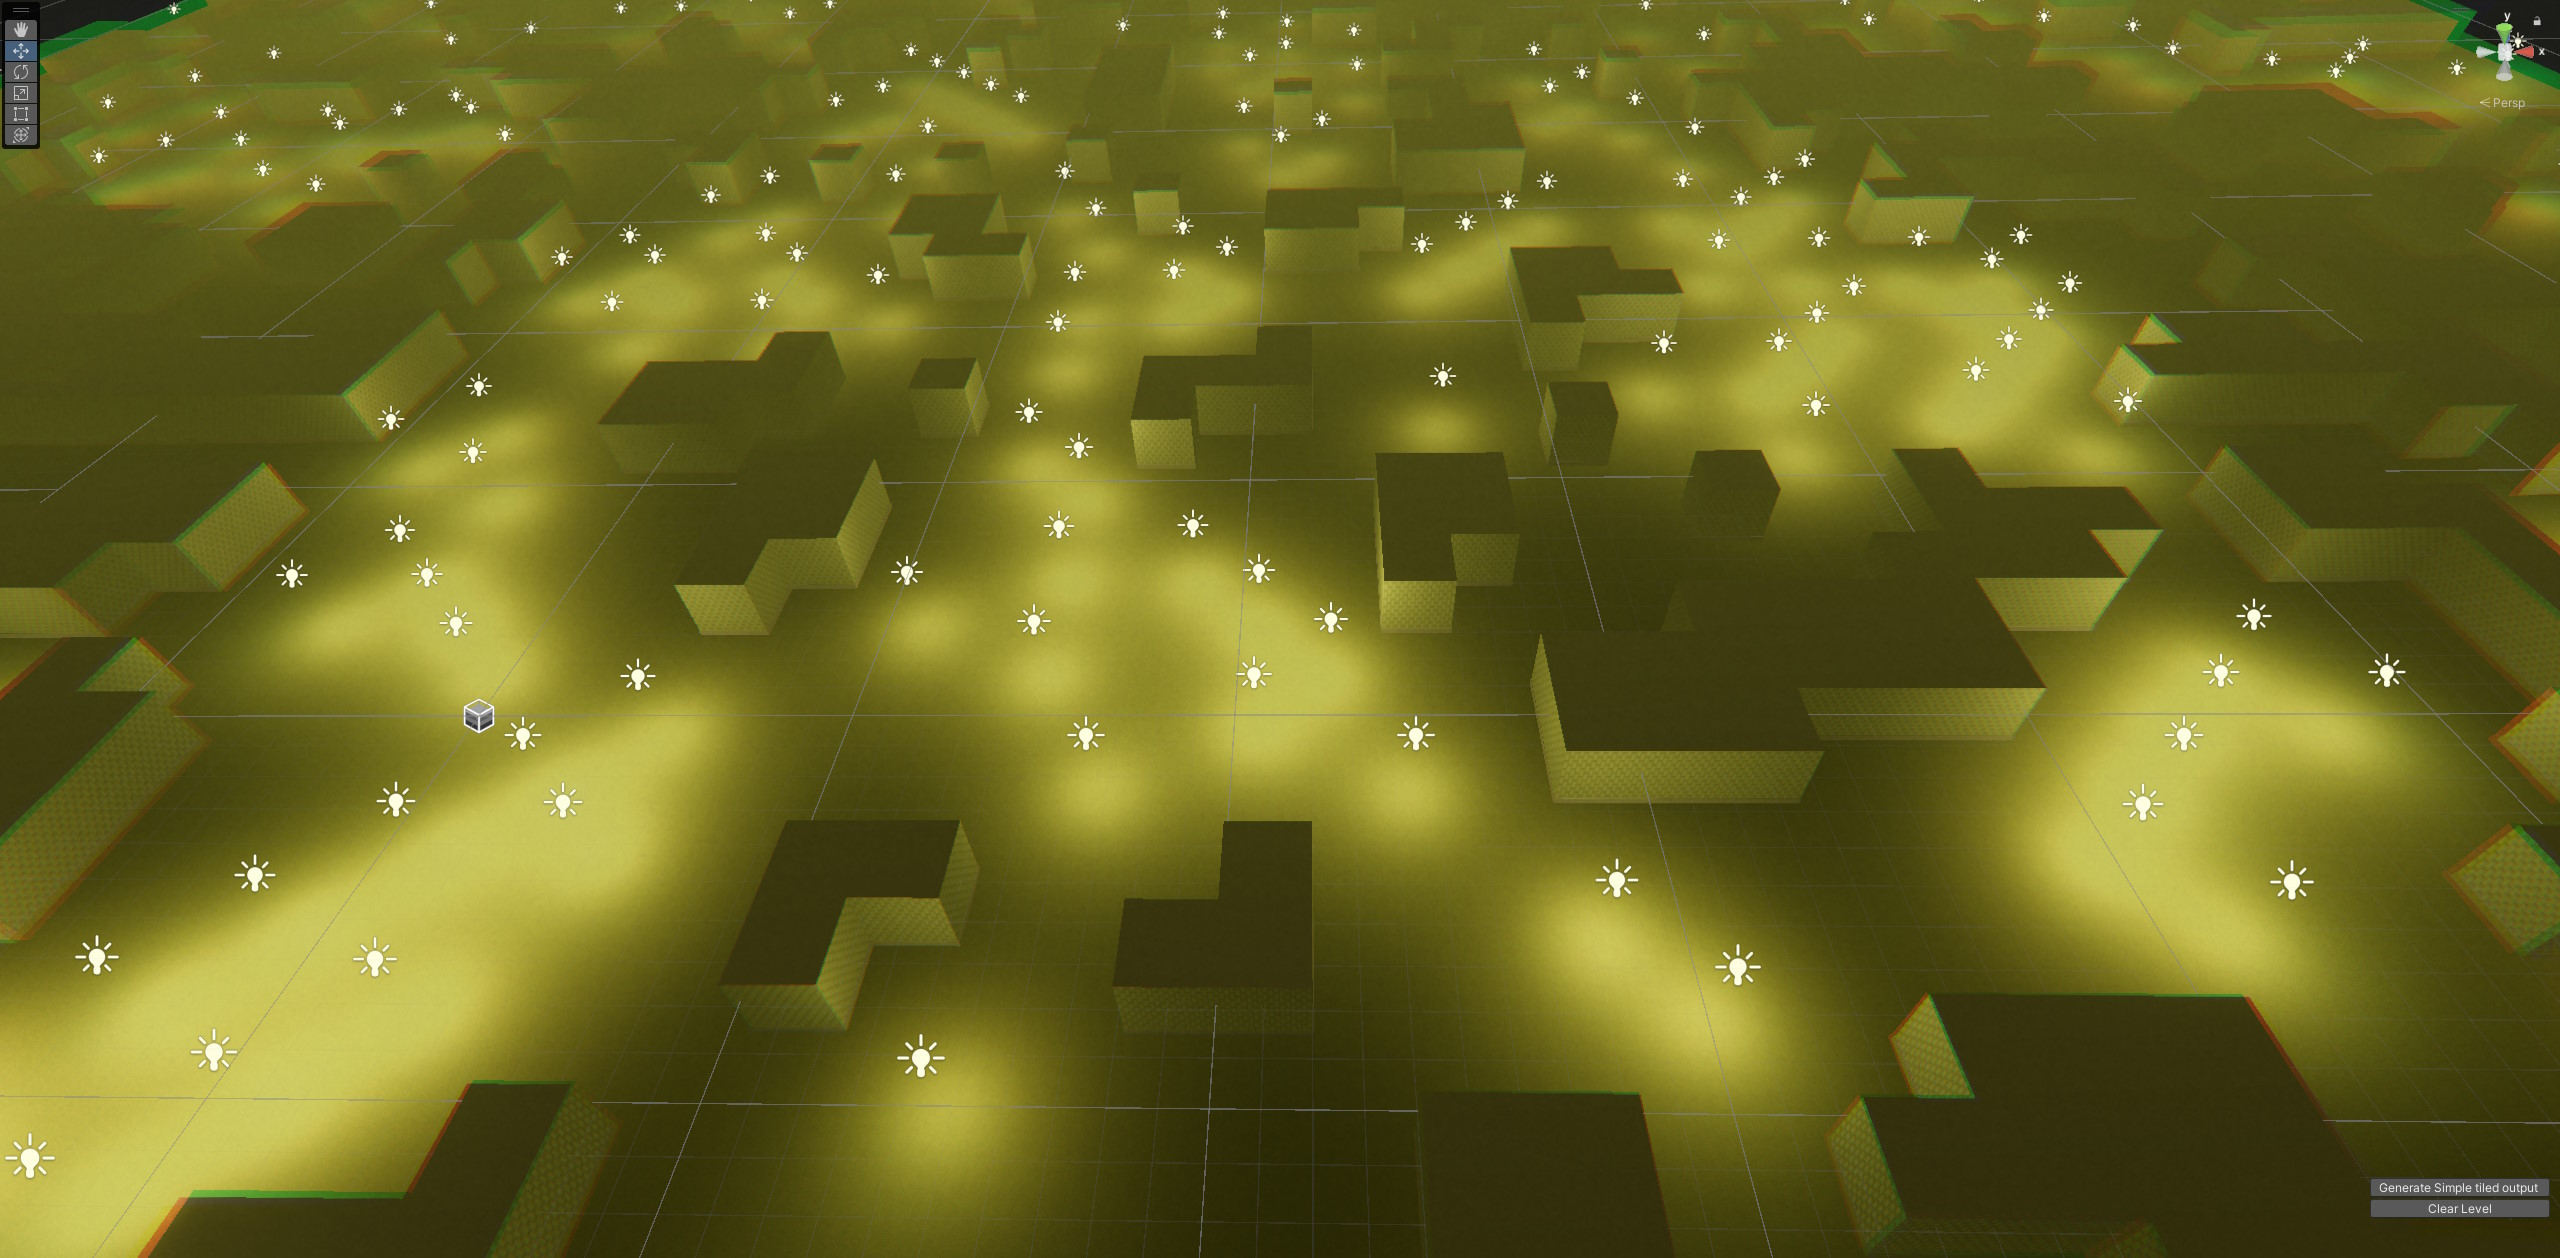
\includegraphics[width=0.975\textwidth, height=0.3\textheight, keepaspectratio]{Images/WeightsNormal.jpg}
        \label{fig:cellSelection3}
    }
    \caption{Examples of levels with three different cell selection techniques}
    \label{fig:cellSelection}
\end{figure}

% Cell selection image. Show how lowest entropy selects the most constrained cell.
%\begin{figure}[H]
%\centering
%\includegraphics[width=\textwidth, height=0.3\textheight, keepaspectratio]{ImagePath}
%\caption{captionText}
%\label{fig:entropyExample}
%\end{figure}

\subsubsection{Weighted Random Tile Selection}
Assigning each tile a weight gives the level designer global control over the percentage of each tile in the output level. Once a cell has been chosen, weighted tile choice is carried out by summing all tile weights and then choosing a random number within that range. This gives higher weight tiles a higher chance to be selected. If the tile choice did not include any randomness, then unplayable levels such as a completely empty level could be generated (Figure \ref{fig:ascendingTileSelection}). In this case, the first tile in the tile set is the empty tile, generating an empty level.

\begin{figure}[H]
    \centering
    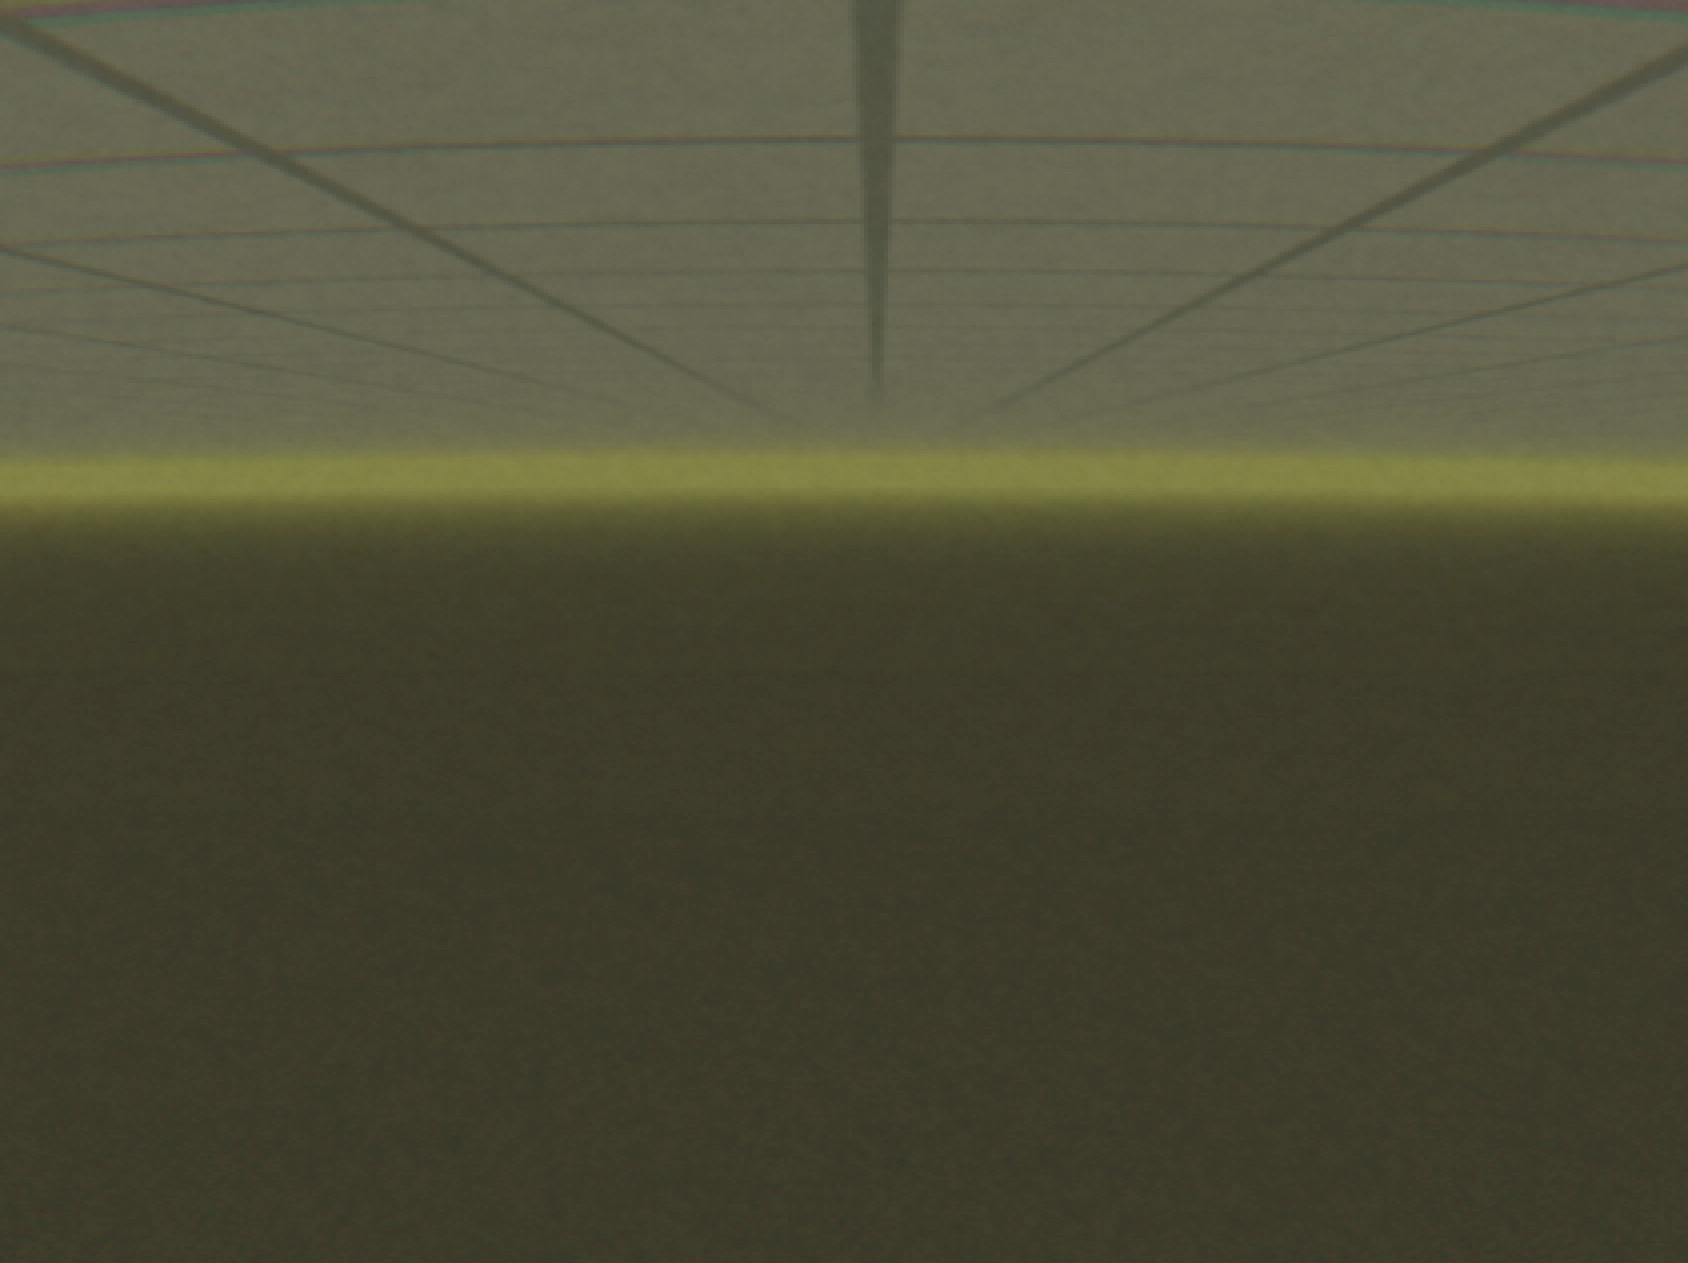
\includegraphics[width=\textwidth, height=0.2\textheight, keepaspectratio]{Images/TileSelectionAscending.jpg}
    \caption{Ascending tile selection has a high chance to generate unplayable levels such as this empty level}
    \label{fig:ascendingTileSelection}
\end{figure}

The chance to generate unplayable levels highlights the challenge in applying a simple constraint solver to level generation in a game. A level that satisfies all constraints for the solver does not necessarily translate to a good level. Some additional constraints could be added in, such as requiring a specific block in generated chunks. However, other constraints such as requiring a certain percentage of a specific block type in the entire level are harder to enforce effectively and efficiently. Such constraints can be encourage implicitly in generation, through features such as the weighted random tile selection. With this, output is not guaranteed to satisfy block percentages, but instead strongly biased towards creating outputs that roughly match these constraints. Figure \ref{fig:weights} shows how different tile weight configurations can create vastly different levels. Careful tweaking of weights is required to create an appealing level. Having too dense of a level can create inaccessible areas as in Figure \ref{fig:weights2}. An alternative tile selection technique is to simply pick tiles at random (Figure \ref{fig:weights4}). This is analogous to giving tiles equal weights. In this case, adjacencies contribute much more to how commonly certain tiles appear.
% Should parts of the above be moved to evaluation or somewhere else?

% Show screenshots of how varying weights produces different levels.
\begin{figure}[H]
    \centering
    \subfigure[Increased weights for empty tiles creates a sparser level]{
        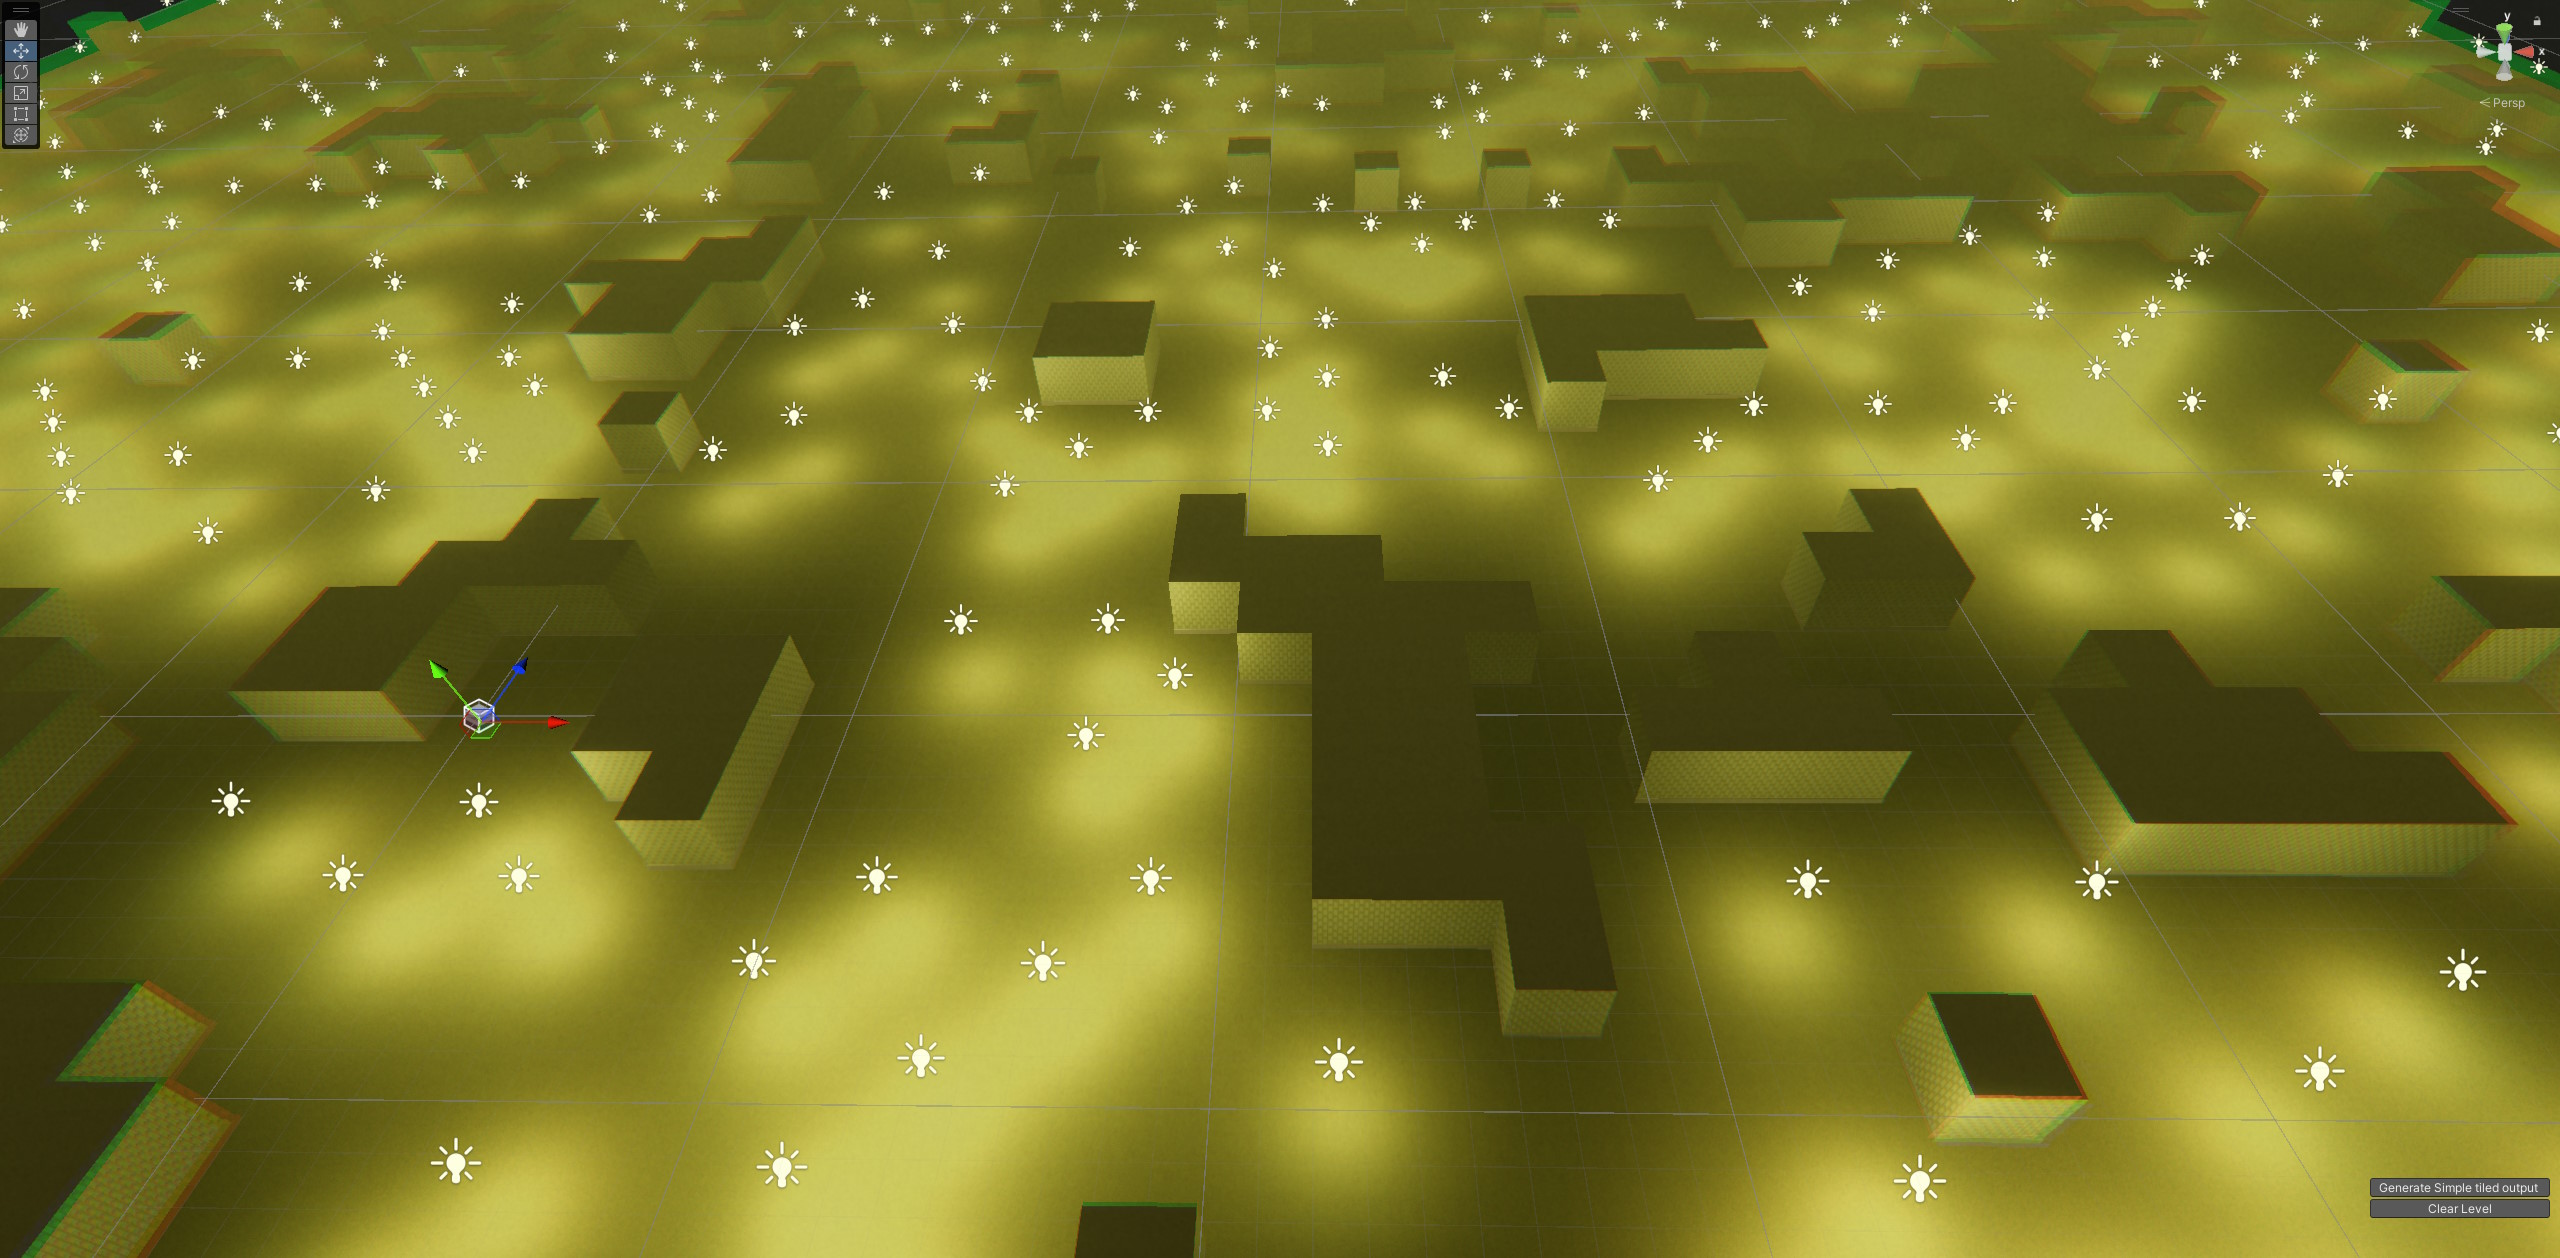
\includegraphics[width=0.475\textwidth, height=0.3\textheight, keepaspectratio]{Images/WeightsSparse.jpg}
        \label{fig:weights1}
    }
    \hfill
    \subfigure[Increasing weights for solid tiles creates a denser level, with increasing chance of unreachable areas]{
        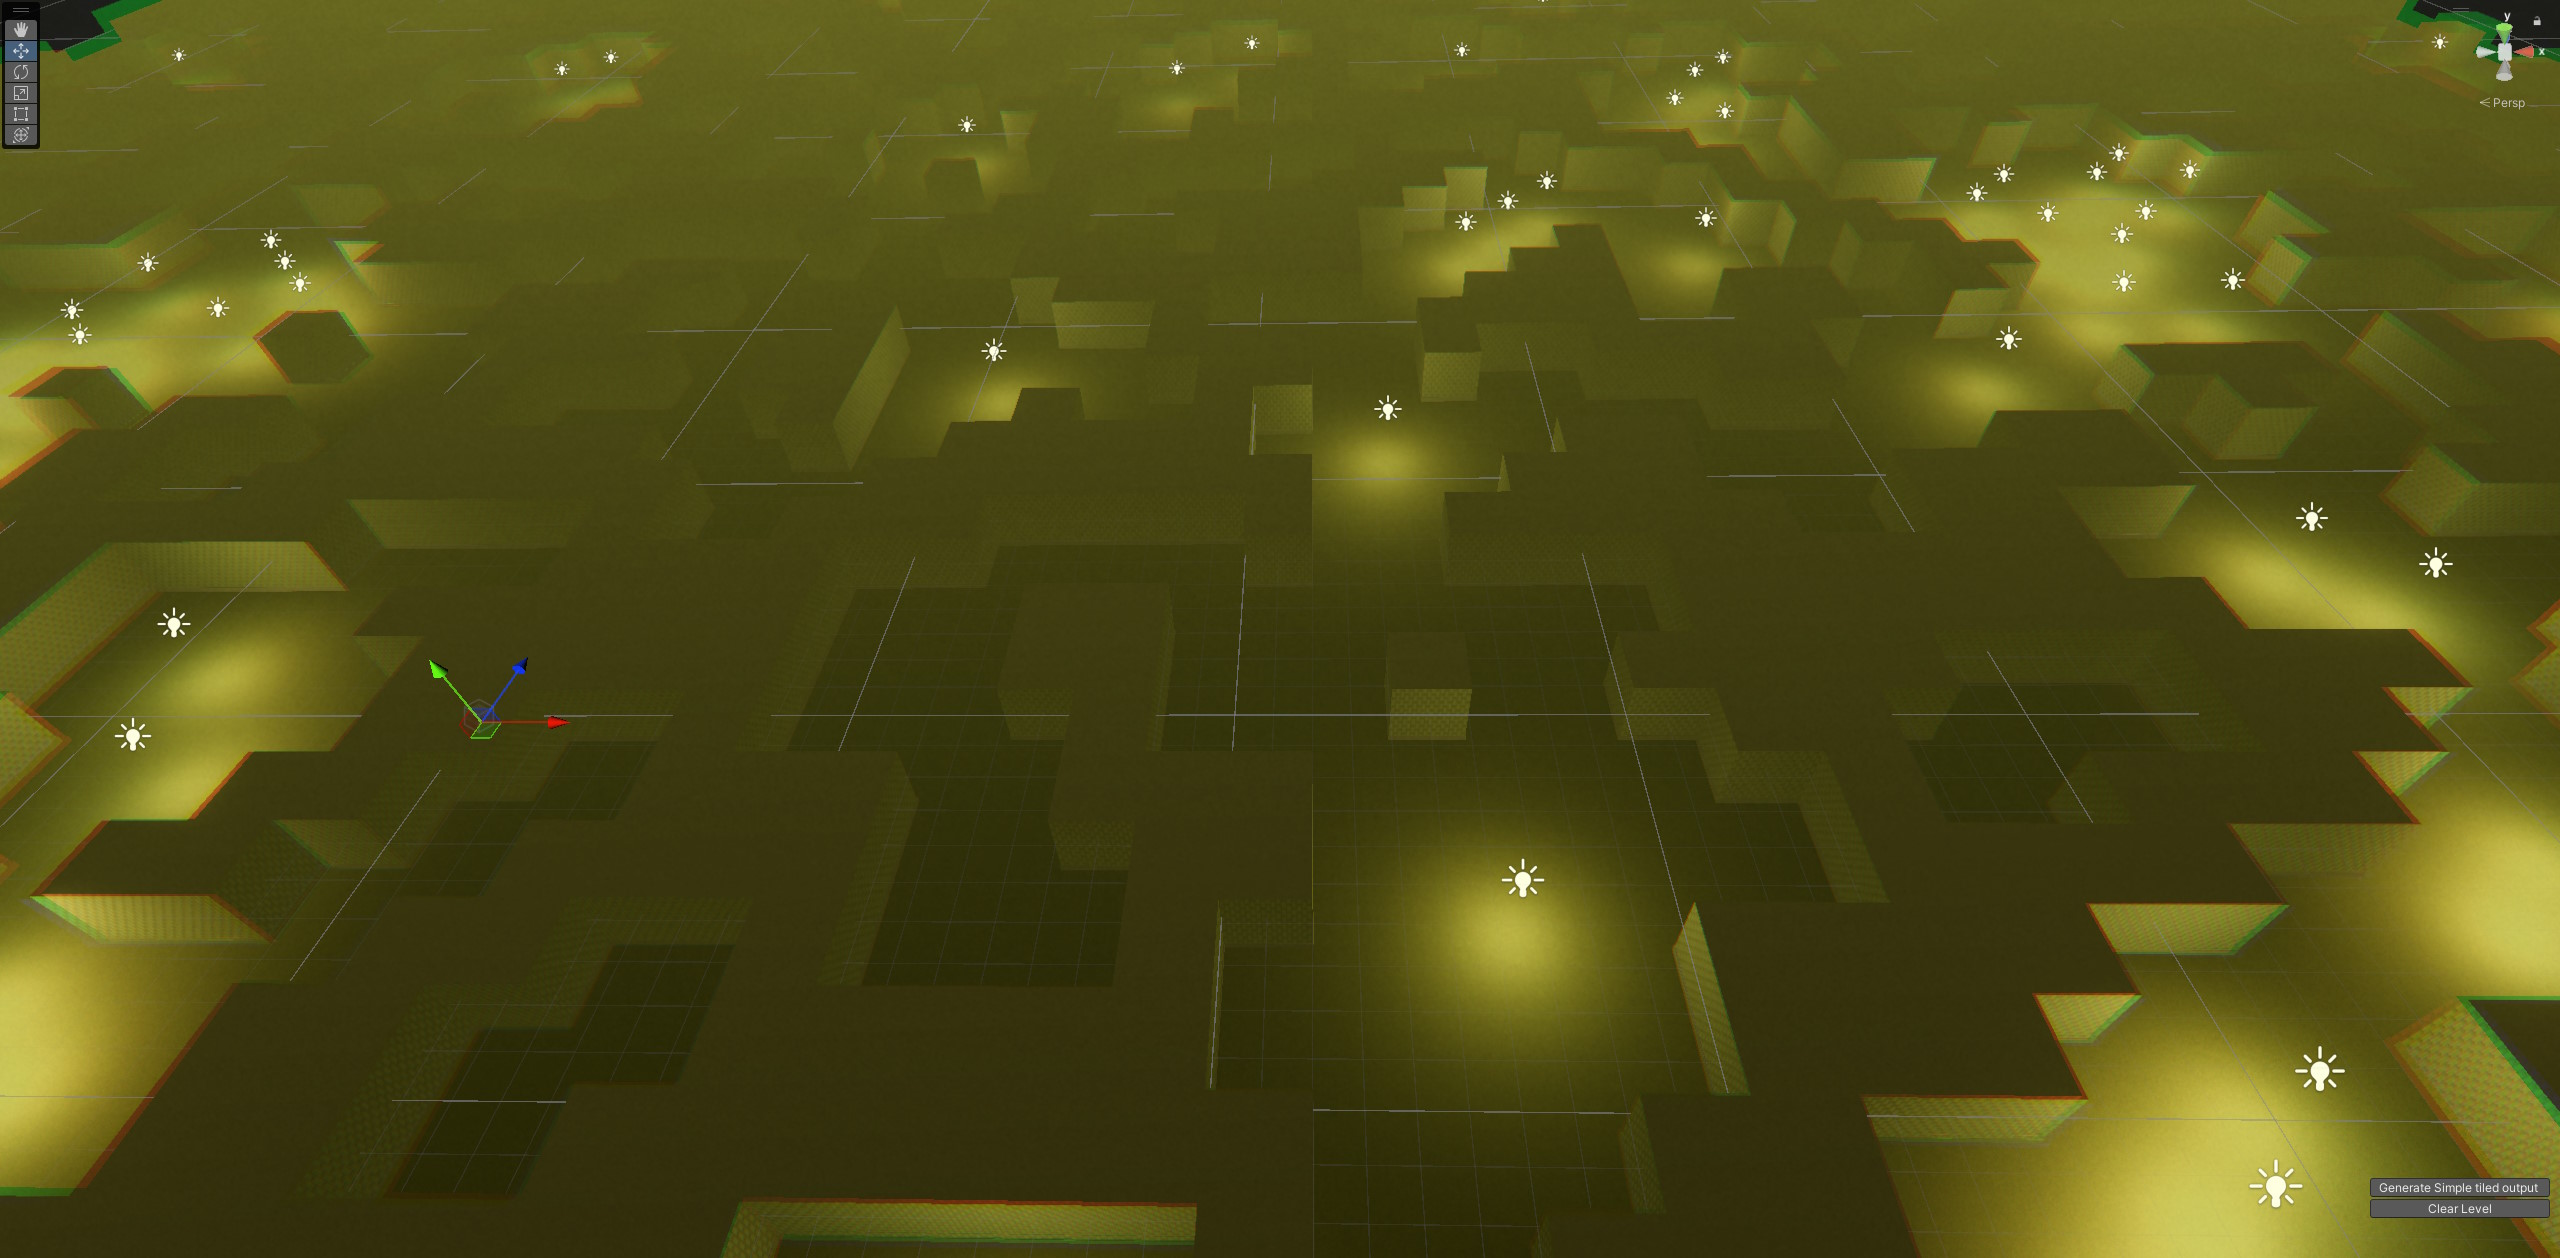
\includegraphics[width=0.475\textwidth, height=0.3\textheight, keepaspectratio]{Images/WeightsDense.jpg}
        \label{fig:weights2}
    }

    \subfigure[A balance of weights for all tiles creates a level with some sparse and some dense areas]{
        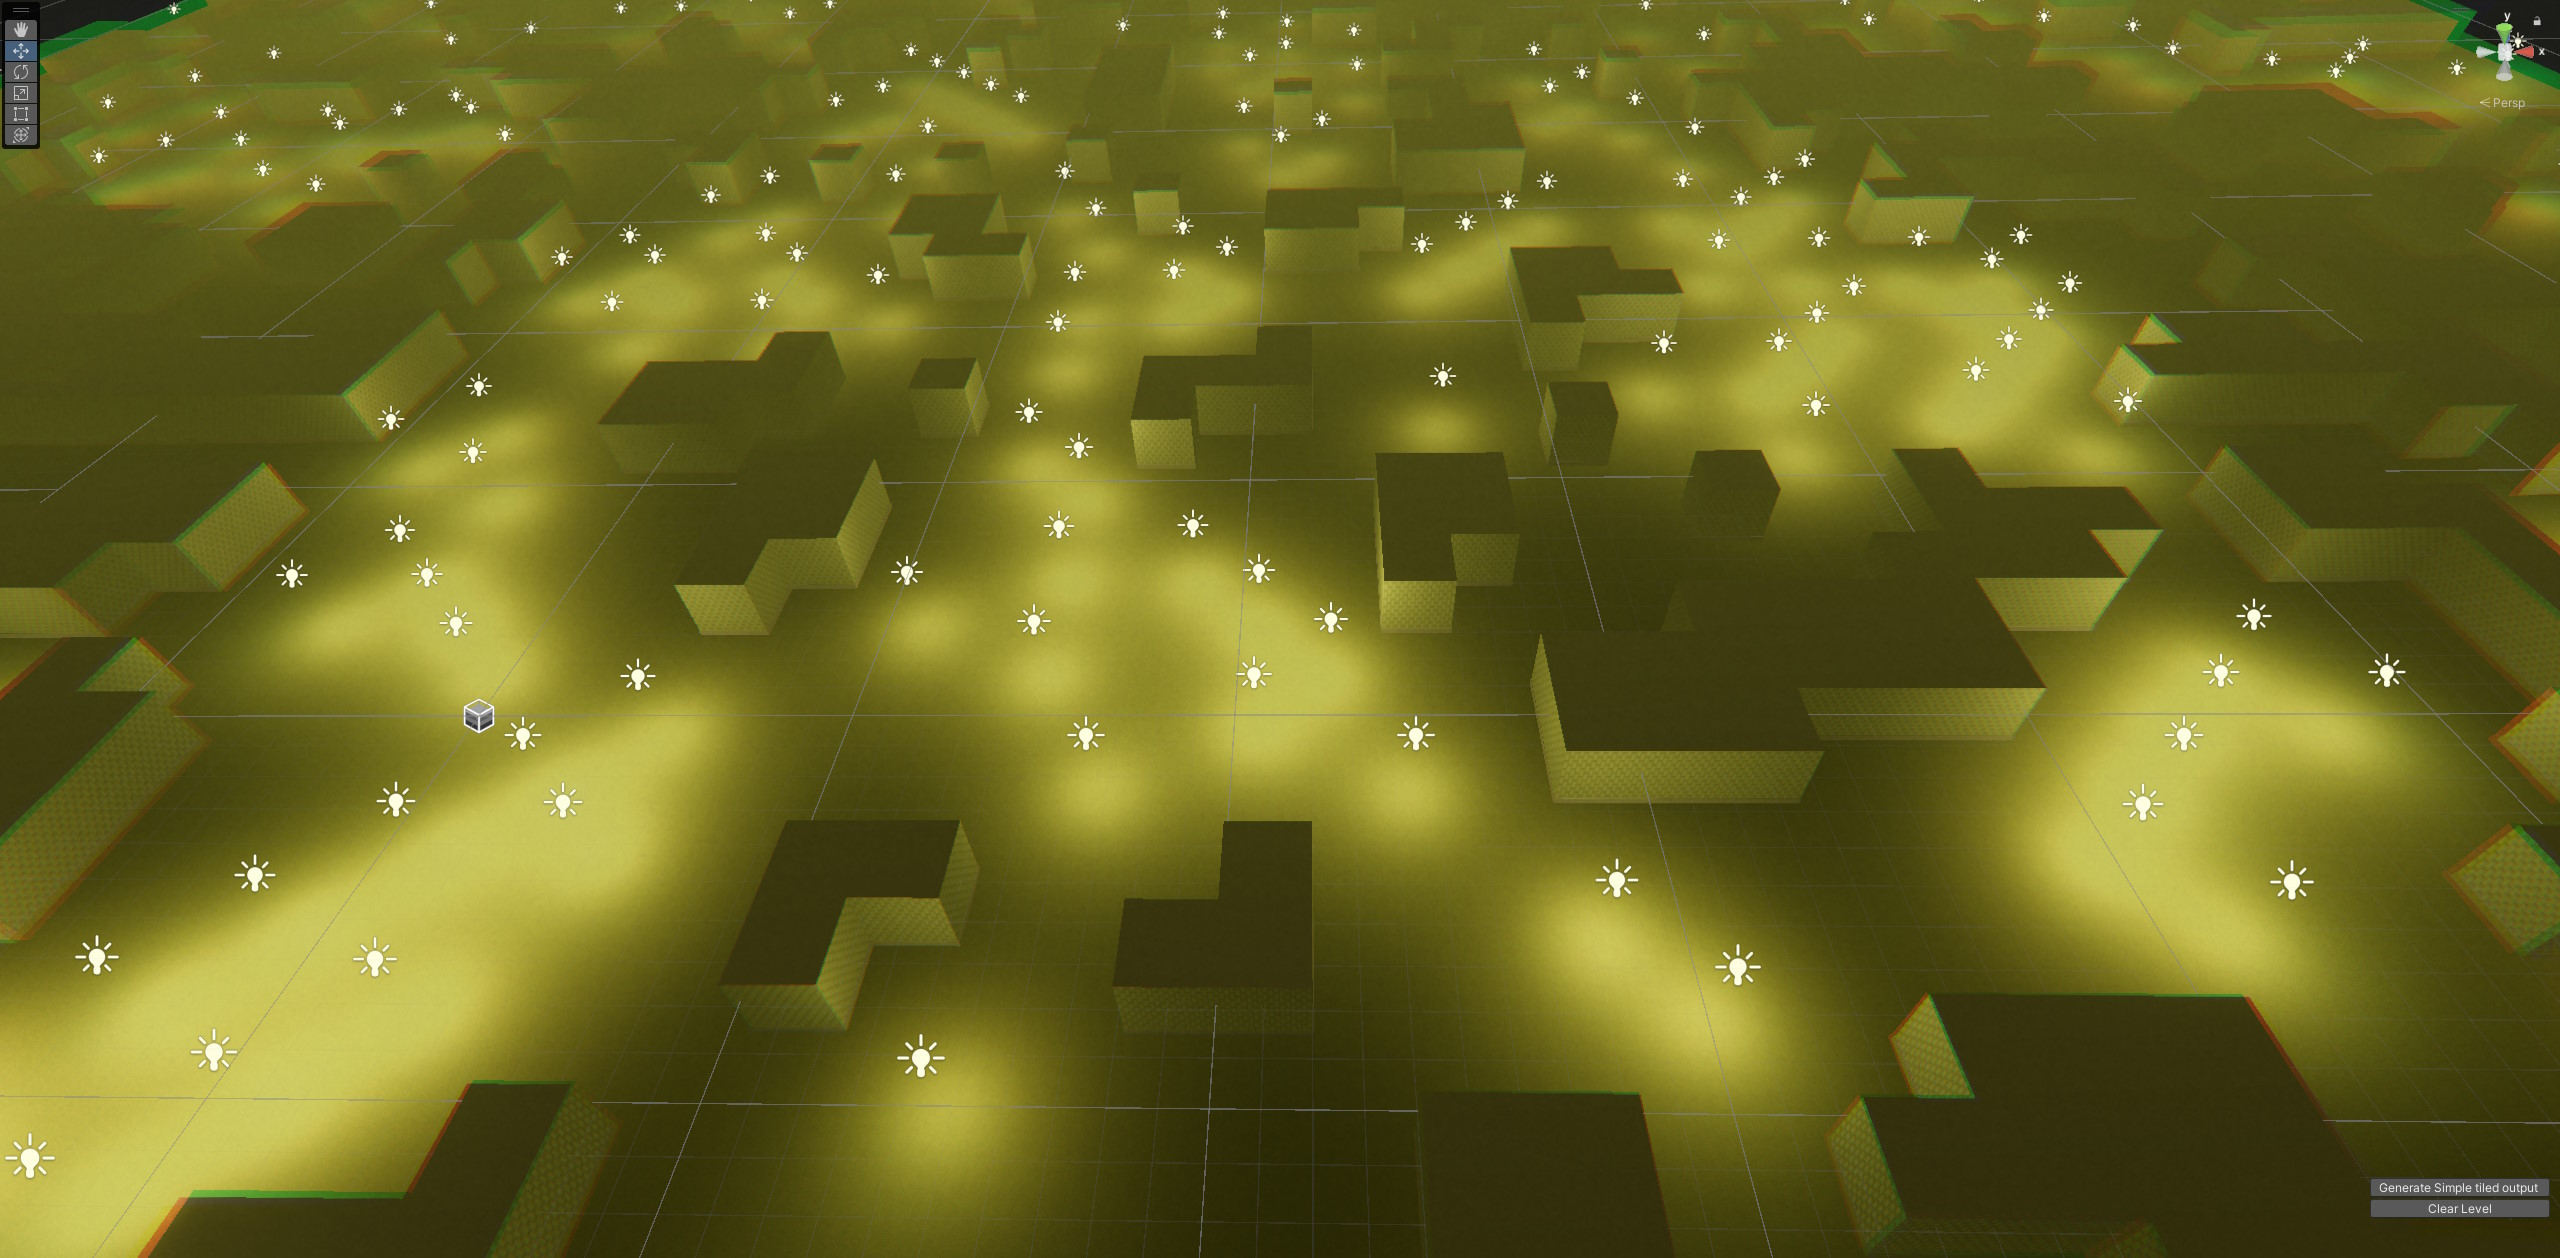
\includegraphics[width=0.475\textwidth, height=0.3\textheight, keepaspectratio]{Images/WeightsNormal.jpg}
        \label{fig:weights3}
    }
    \hfill
    \subfigure[Having equal weights (randomly selecting tiles) gives less control over tile percentages]{
        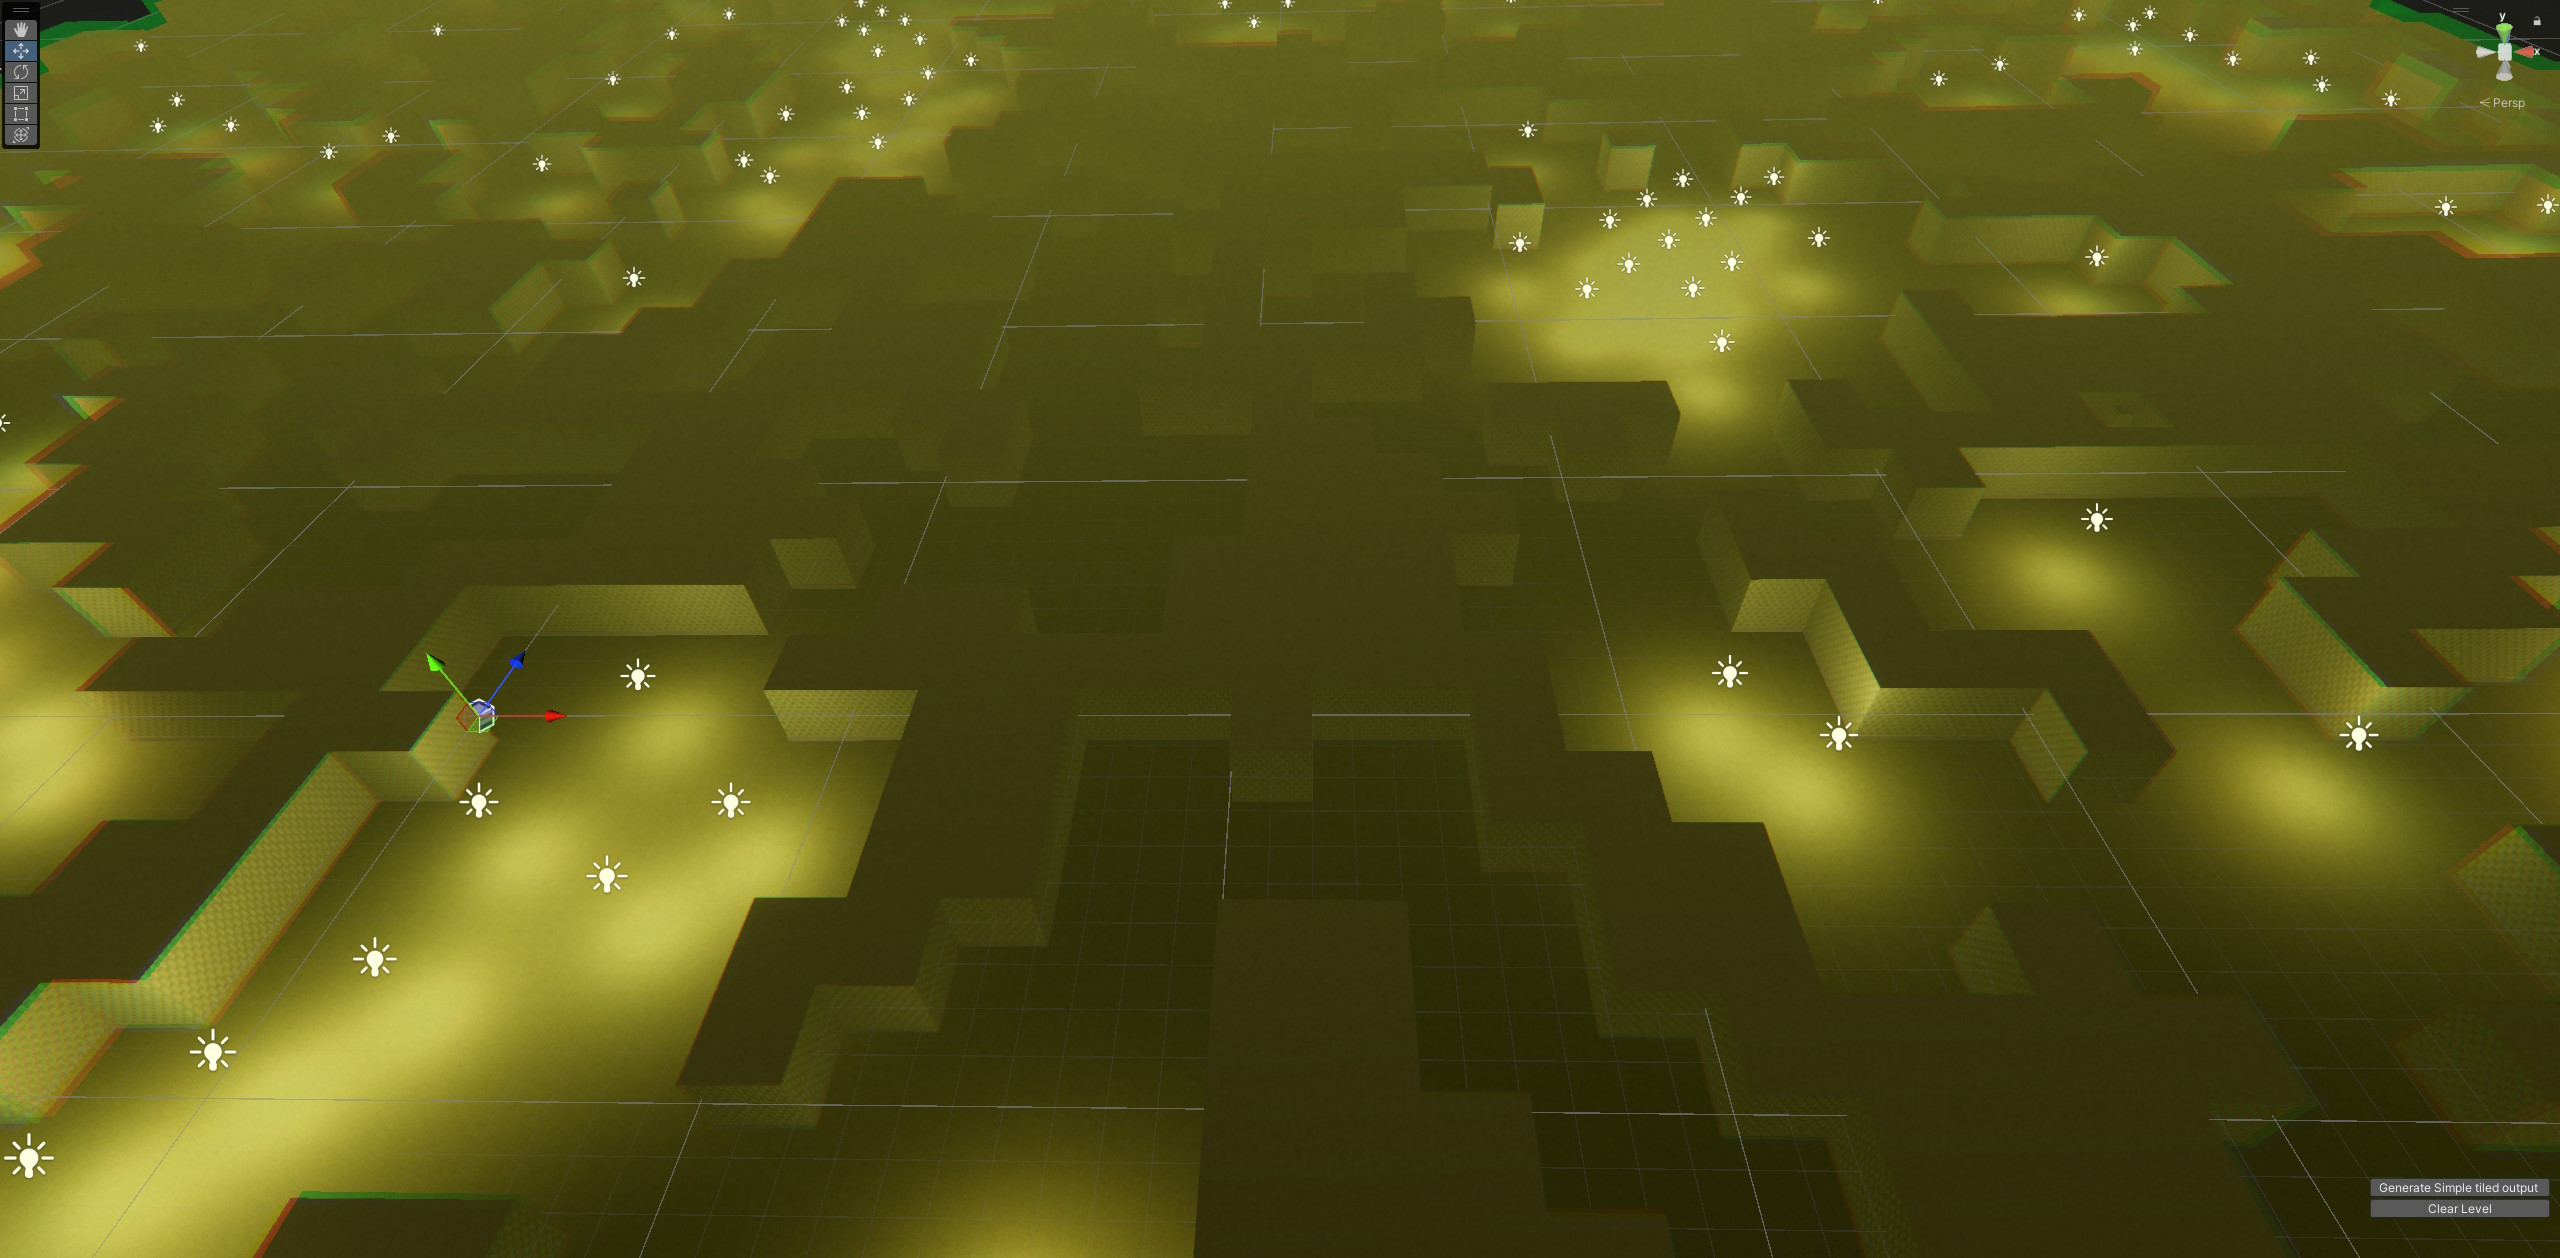
\includegraphics[width=0.475\textwidth, height=0.3\textheight, keepaspectratio]{Images/TileSelectionRandom.jpg}
        \label{fig:weights4}
    }
    \caption{Examples of levels with four different tile weight configurations}
    \label{fig:weights}
\end{figure}

\subsection{Infinite Modifying in Blocks}
\label{sec:IMIB}
\acrlong{imib} works by splitting up generation into overlapping chunks, each of which are split into four layers. These layers are offset such that they do not interfere with each other. This can be used to ensure that generation is deterministic and optionally process each layer in parallel. As example, Figure \ref{fig:imibChunkComparison1} shows how a single chunk is formed of four overlapping layers. Extending on this, Figure \ref{fig:imibChunkComparison2} shows how chunks overlap with each other, highlighting the layers of another chunk in lighter colours. The images from the original source were edited to show more clearly the concepts of chunks and layers as implemented.

% Diagram of chunks.
\begin{figure}[H]
    \centering
    \subfigure[The four layers making up a single chunk]{
        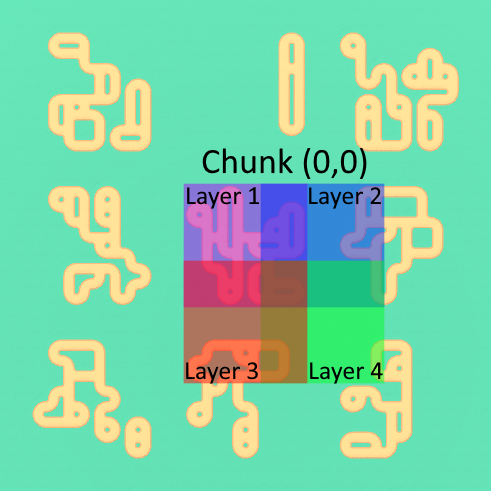
\includegraphics[width=0.475\textwidth, height=0.3\textheight, keepaspectratio]{Images/IMIB Comparison Single Chunk.png}
        \label{fig:imibChunkComparison1}
    }
    \hfill
    \subfigure[Overlap between adjacent chunks]{
        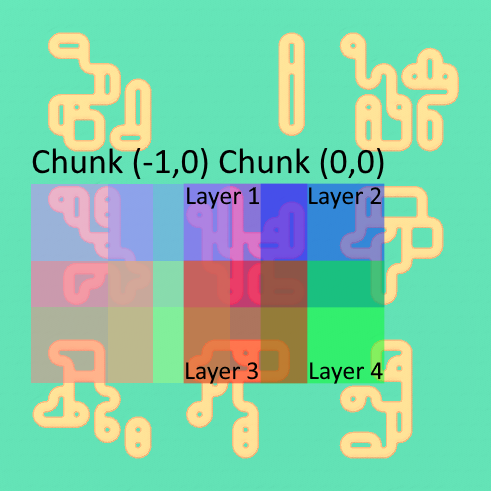
\includegraphics[width=0.475\textwidth, height=0.3\textheight, keepaspectratio]{Images/IMIB Comparison Two Chunks.png}
        \label{fig:imibChunkComparison2}
    }
    \caption{\acrshort{imib} uses a grid of overlapping chunks consisting of overlapping layers}
    \label{fig:imibChunkComparison}
\end{figure}

The algorithm is run layer by layer, finishing the layers of all active chunks before moving to the next layer. First, a layer is prepared. This involves calculating the area inside of the chunk that forms the layer and clearing all cells inside of it (Figure \ref{fig:imibLayerOne1}). Second, the solver tries to find a solution for the layer (Figure \ref{fig:imibLayerOne2}). This takes into account adjacency information from the cells next to the layer. If a solution is not found, the layer is left as it was before. This is not an issue for most tile sets as single layer failures are hidden by other layers successfully generating.

% Show first layer preparation and single layer generated.
\begin{figure}[H]
    \centering
    \subfigure[The first layer is defined and cleared]{
        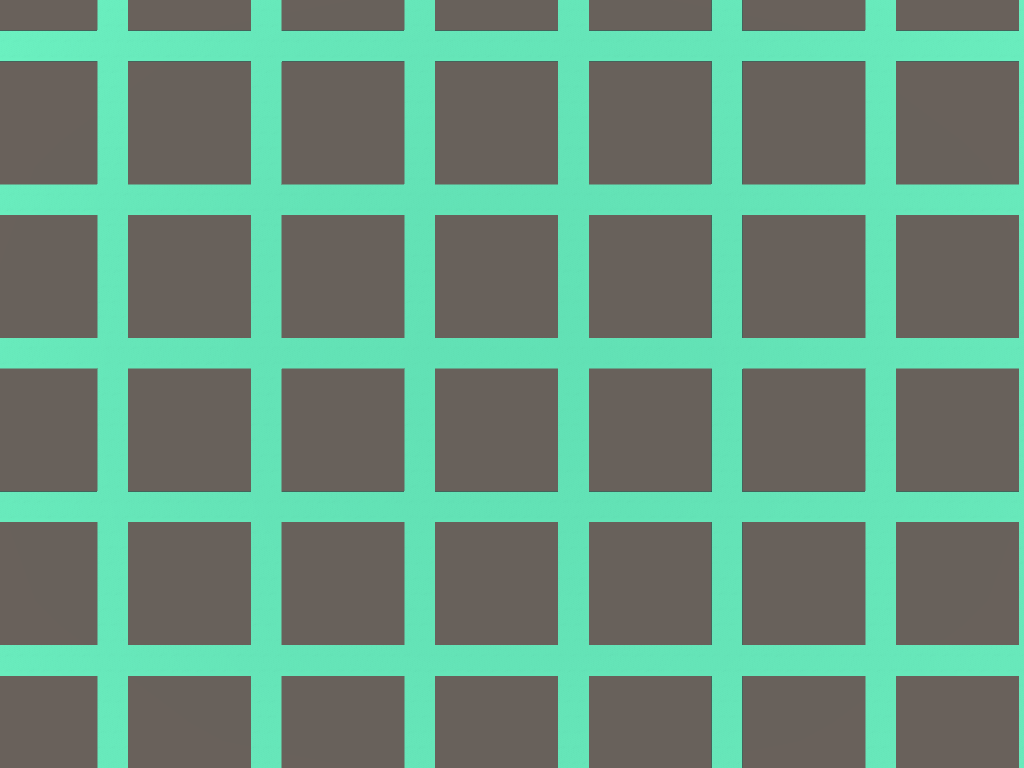
\includegraphics[width=0.475\textwidth, height=0.3\textheight, keepaspectratio]{Images/IMIB2.png}
        \label{fig:imibLayerOne1}
    }
    \hfill
    \subfigure[The first layer is generated]{
        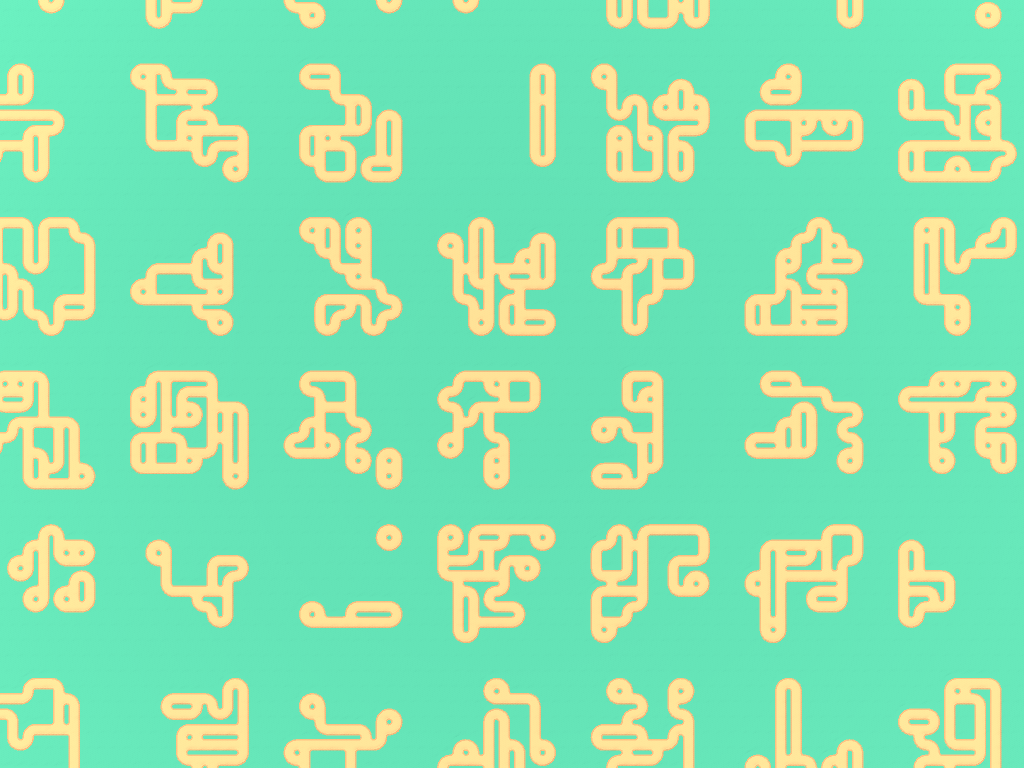
\includegraphics[width=0.475\textwidth, height=0.3\textheight, keepaspectratio]{Images/IMIB3.png}
        \label{fig:imibLayerOne2}
    }
    \caption{Clearing and generating layer 1 as part of \acrshort{imib}}
    \label{fig:imibLayerOne}
\end{figure}

Once each chunk has generated its first layer, the second layer is cleared (Figure \ref{fig:imibLayerTwo1}) and generated (Figure \ref{fig:imibLayerTwo2}). This process is repeated until all layers have been generated (Figure \ref{fig:imibLayerTwo3}).

% Images of all layers generating.
\begin{figure}[H]
    \centering
    \subfigure[The second layer is defined and cleared]{
        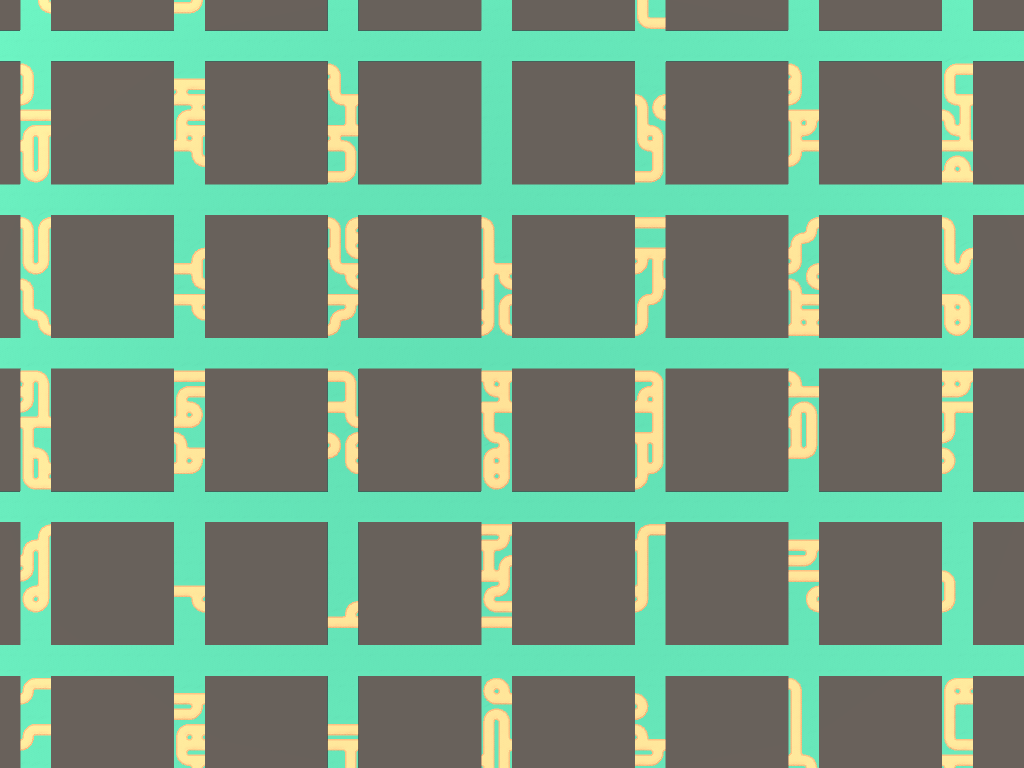
\includegraphics[width=0.475\textwidth, height=0.3\textheight, keepaspectratio]{Images/IMIB4.png}
        \label{fig:imibLayerTwo1}
    }
    \hfill
    \subfigure[The second layer is generated]{
        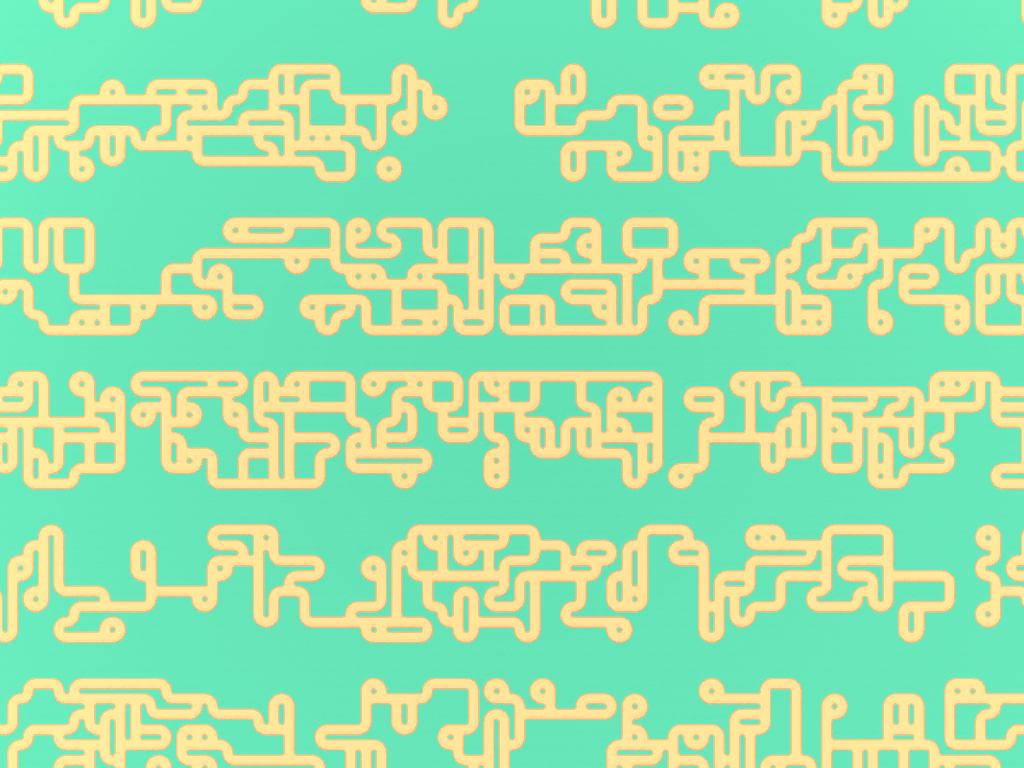
\includegraphics[width=0.475\textwidth, height=0.3\textheight, keepaspectratio]{Images/IMIB5.png}
        \label{fig:imibLayerTwo2}
    }

    \subfigure[The result after all layers have been generated]{
        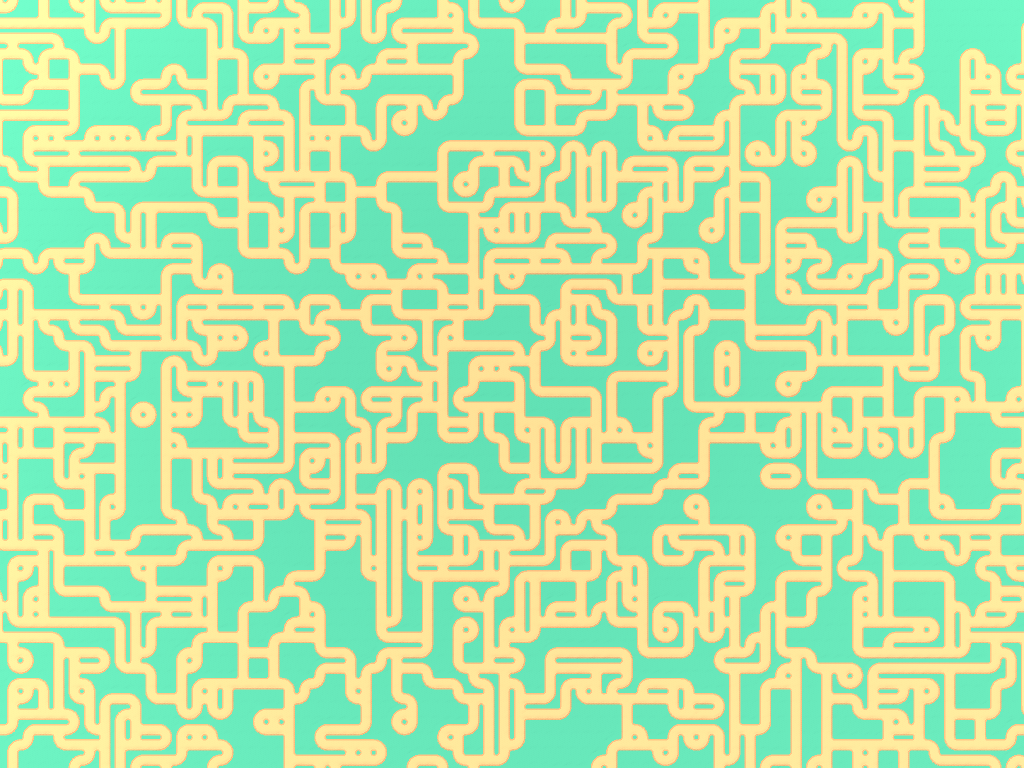
\includegraphics[width=0.975\textwidth, height=0.3\textheight, keepaspectratio]{Images/IMIB9.png}
        \label{fig:imibLayerTwo3}
    }
    \caption{Each \acrshort{imib} layer is generated in turn to compose a full result}
    \label{fig:imibLayerTwo}
\end{figure}

As further example, Figure \ref{fig:backroomsIMIB} shows \acrshort{imib} applies with \textit{the Backrooms} tile set.

\begin{figure}[H]
    \centering
    \subfigure[Generation of layer 1]{
        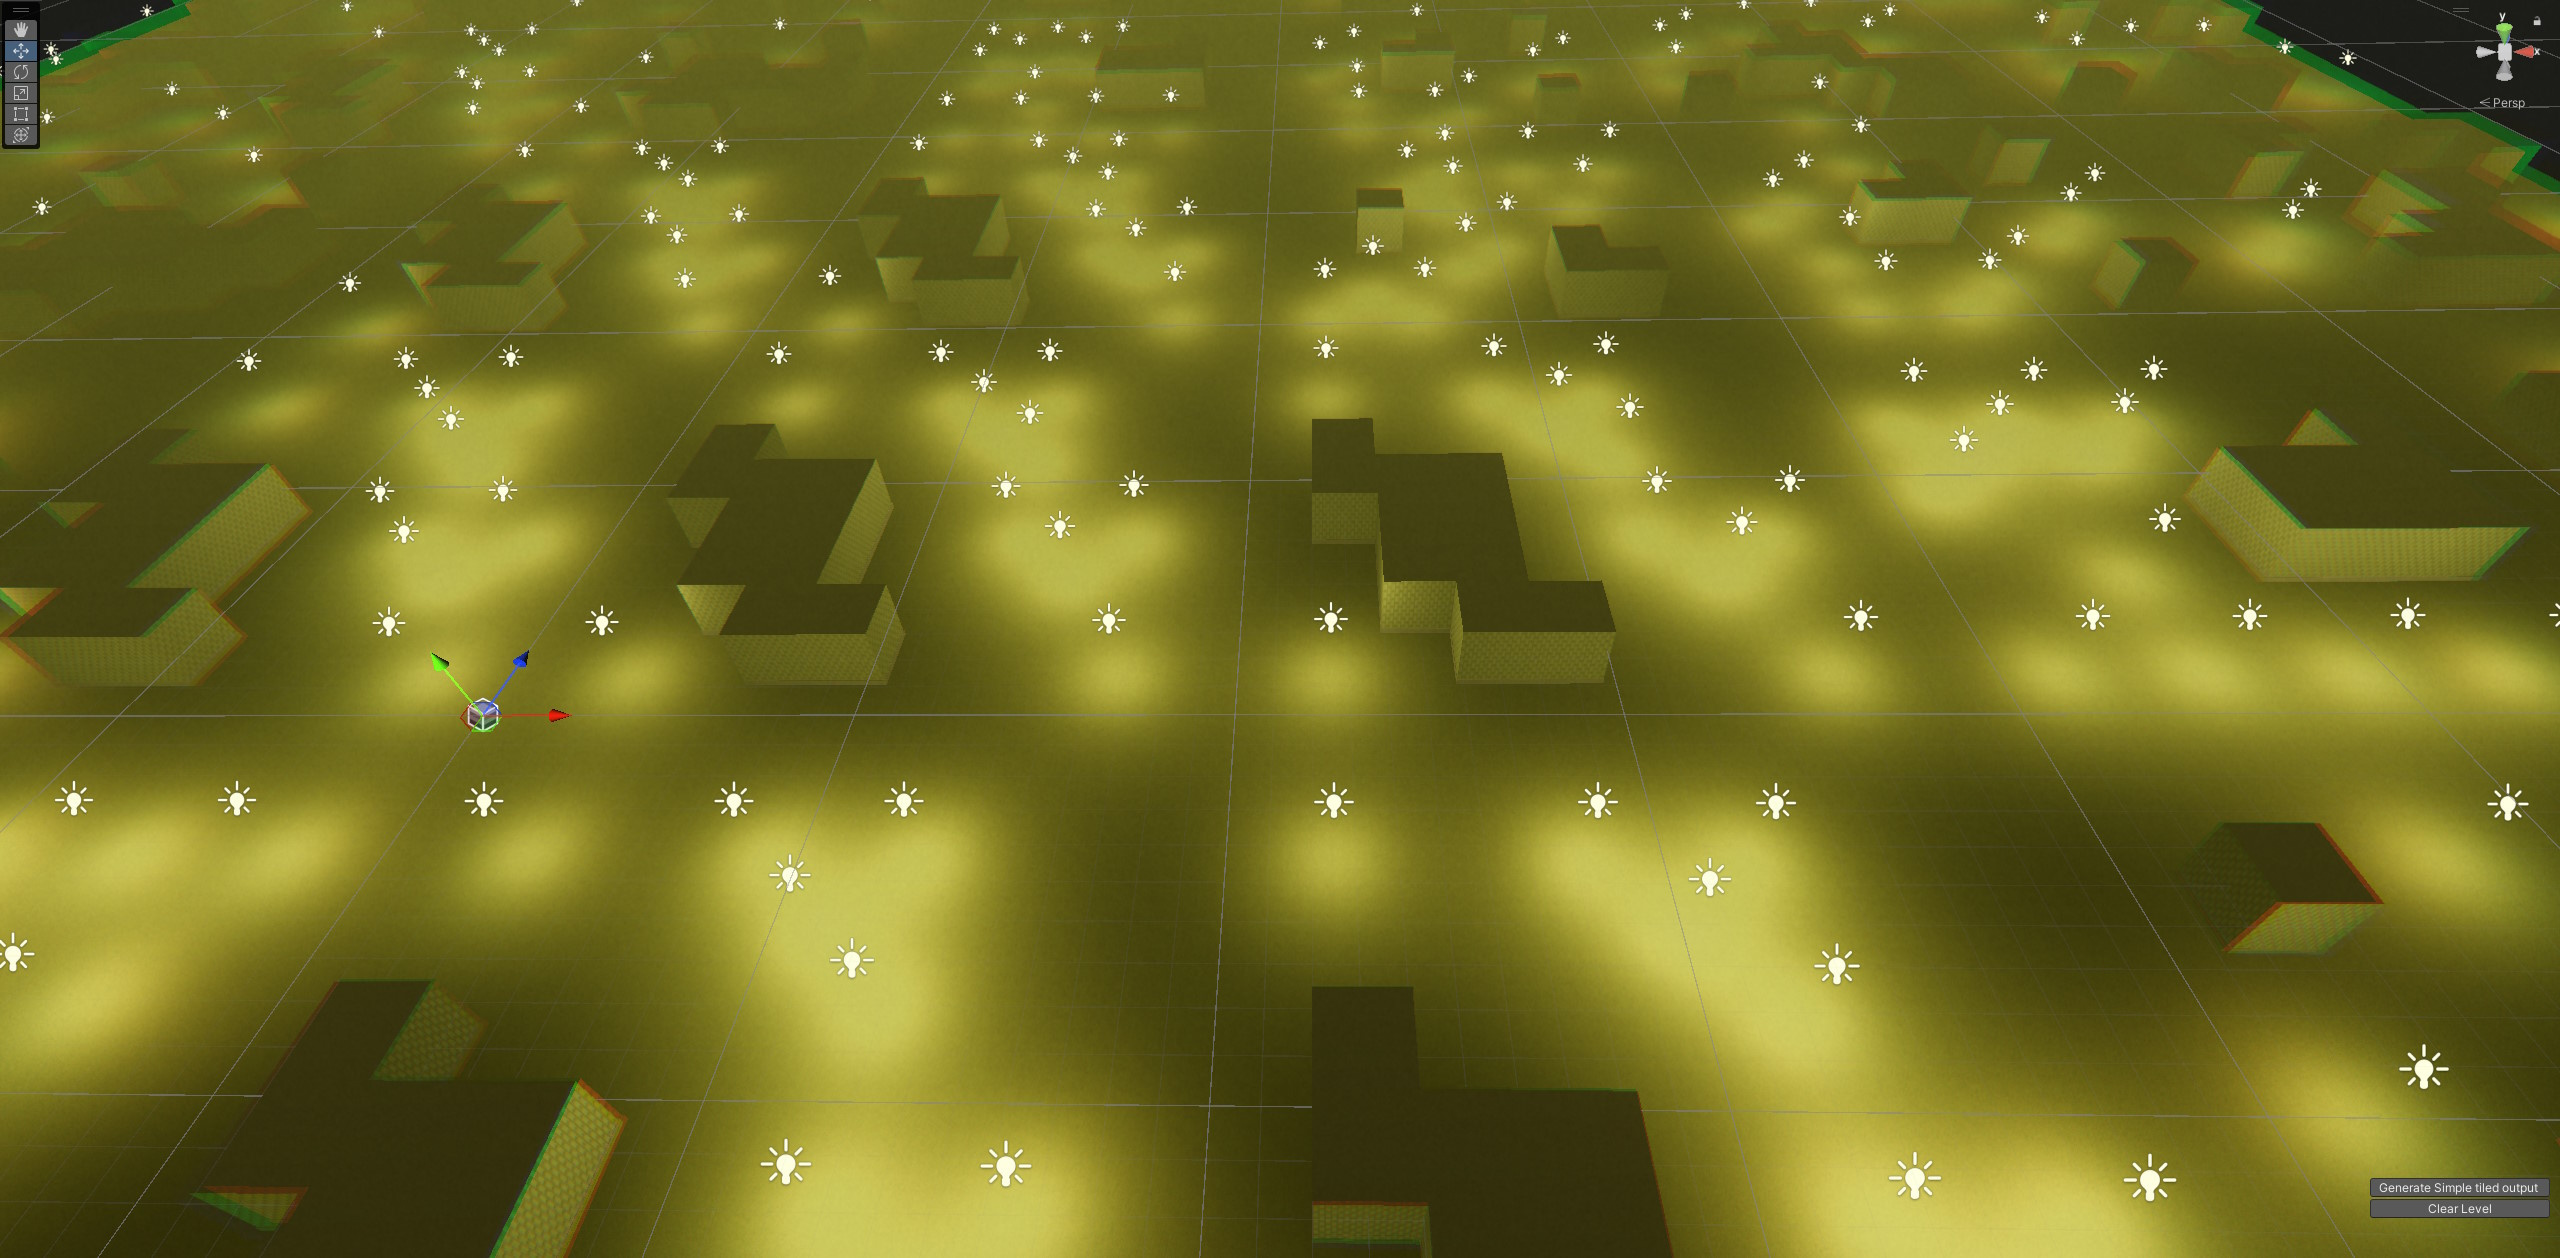
\includegraphics[width=0.475\textwidth, height=0.2\textheight, keepaspectratio]{Images/BackroomsIMIB1.jpg}
        \label{fig:backroomsIMIB1}
    }
    \hfill
    \subfigure[Generation of layer 2]{
        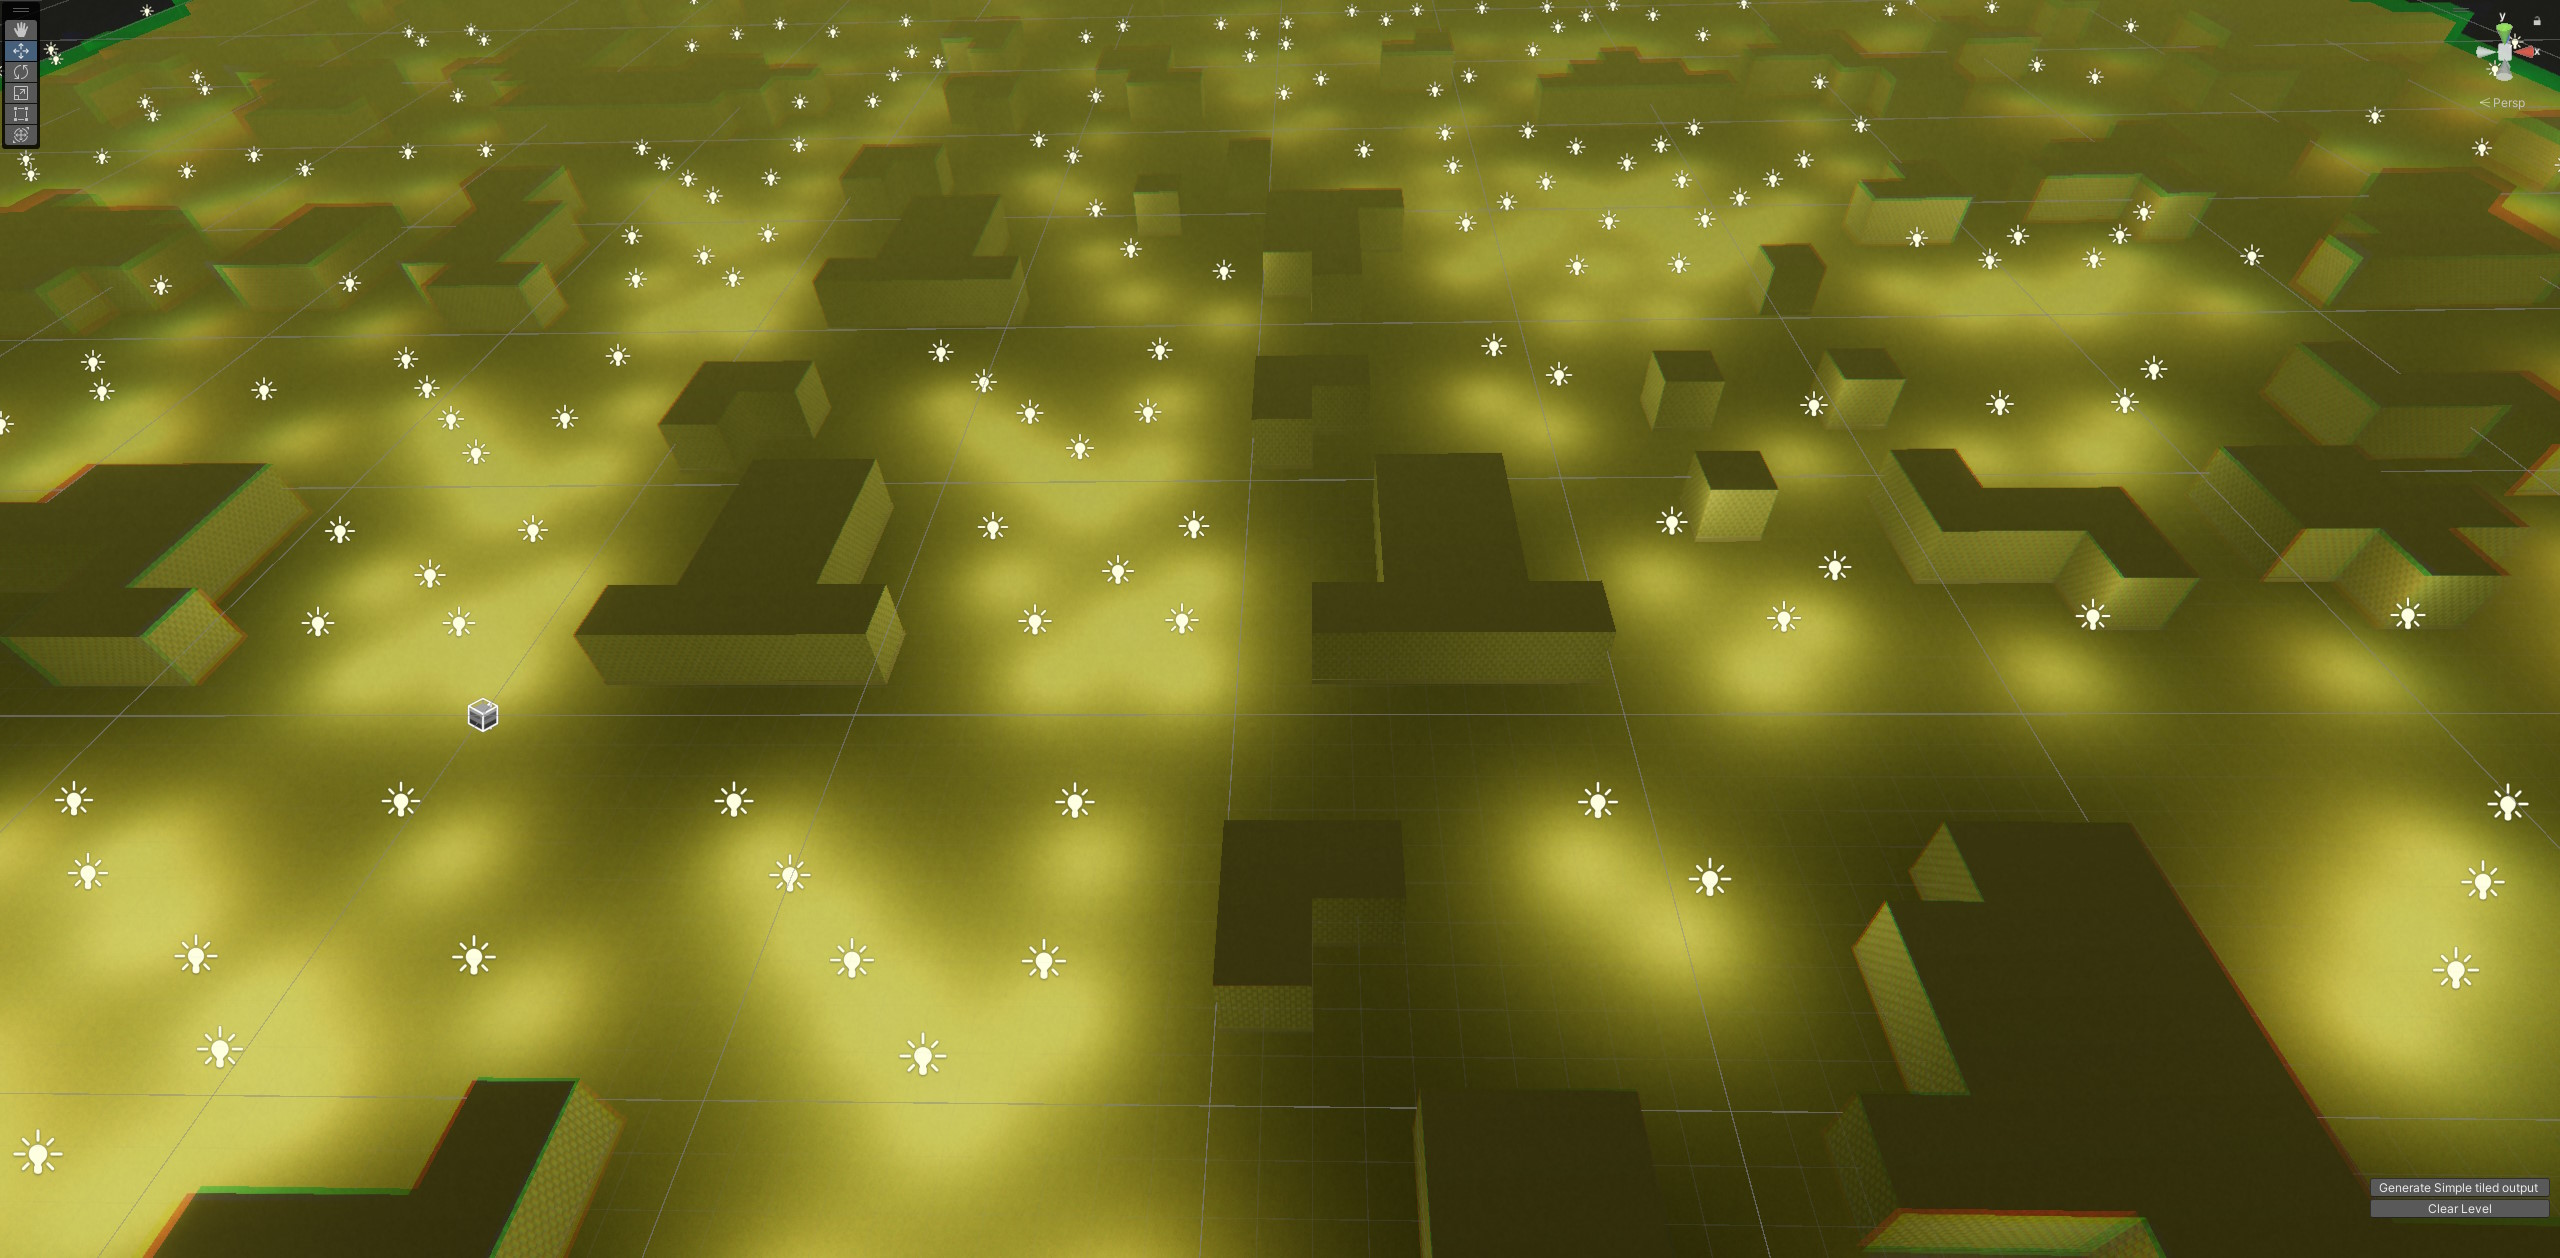
\includegraphics[width=0.475\textwidth, height=0.2\textheight, keepaspectratio]{Images/BackroomsIMIB2.jpg}
        \label{fig:backroomsIMIB2}
    }

    \subfigure[Generation of layer 3]{
        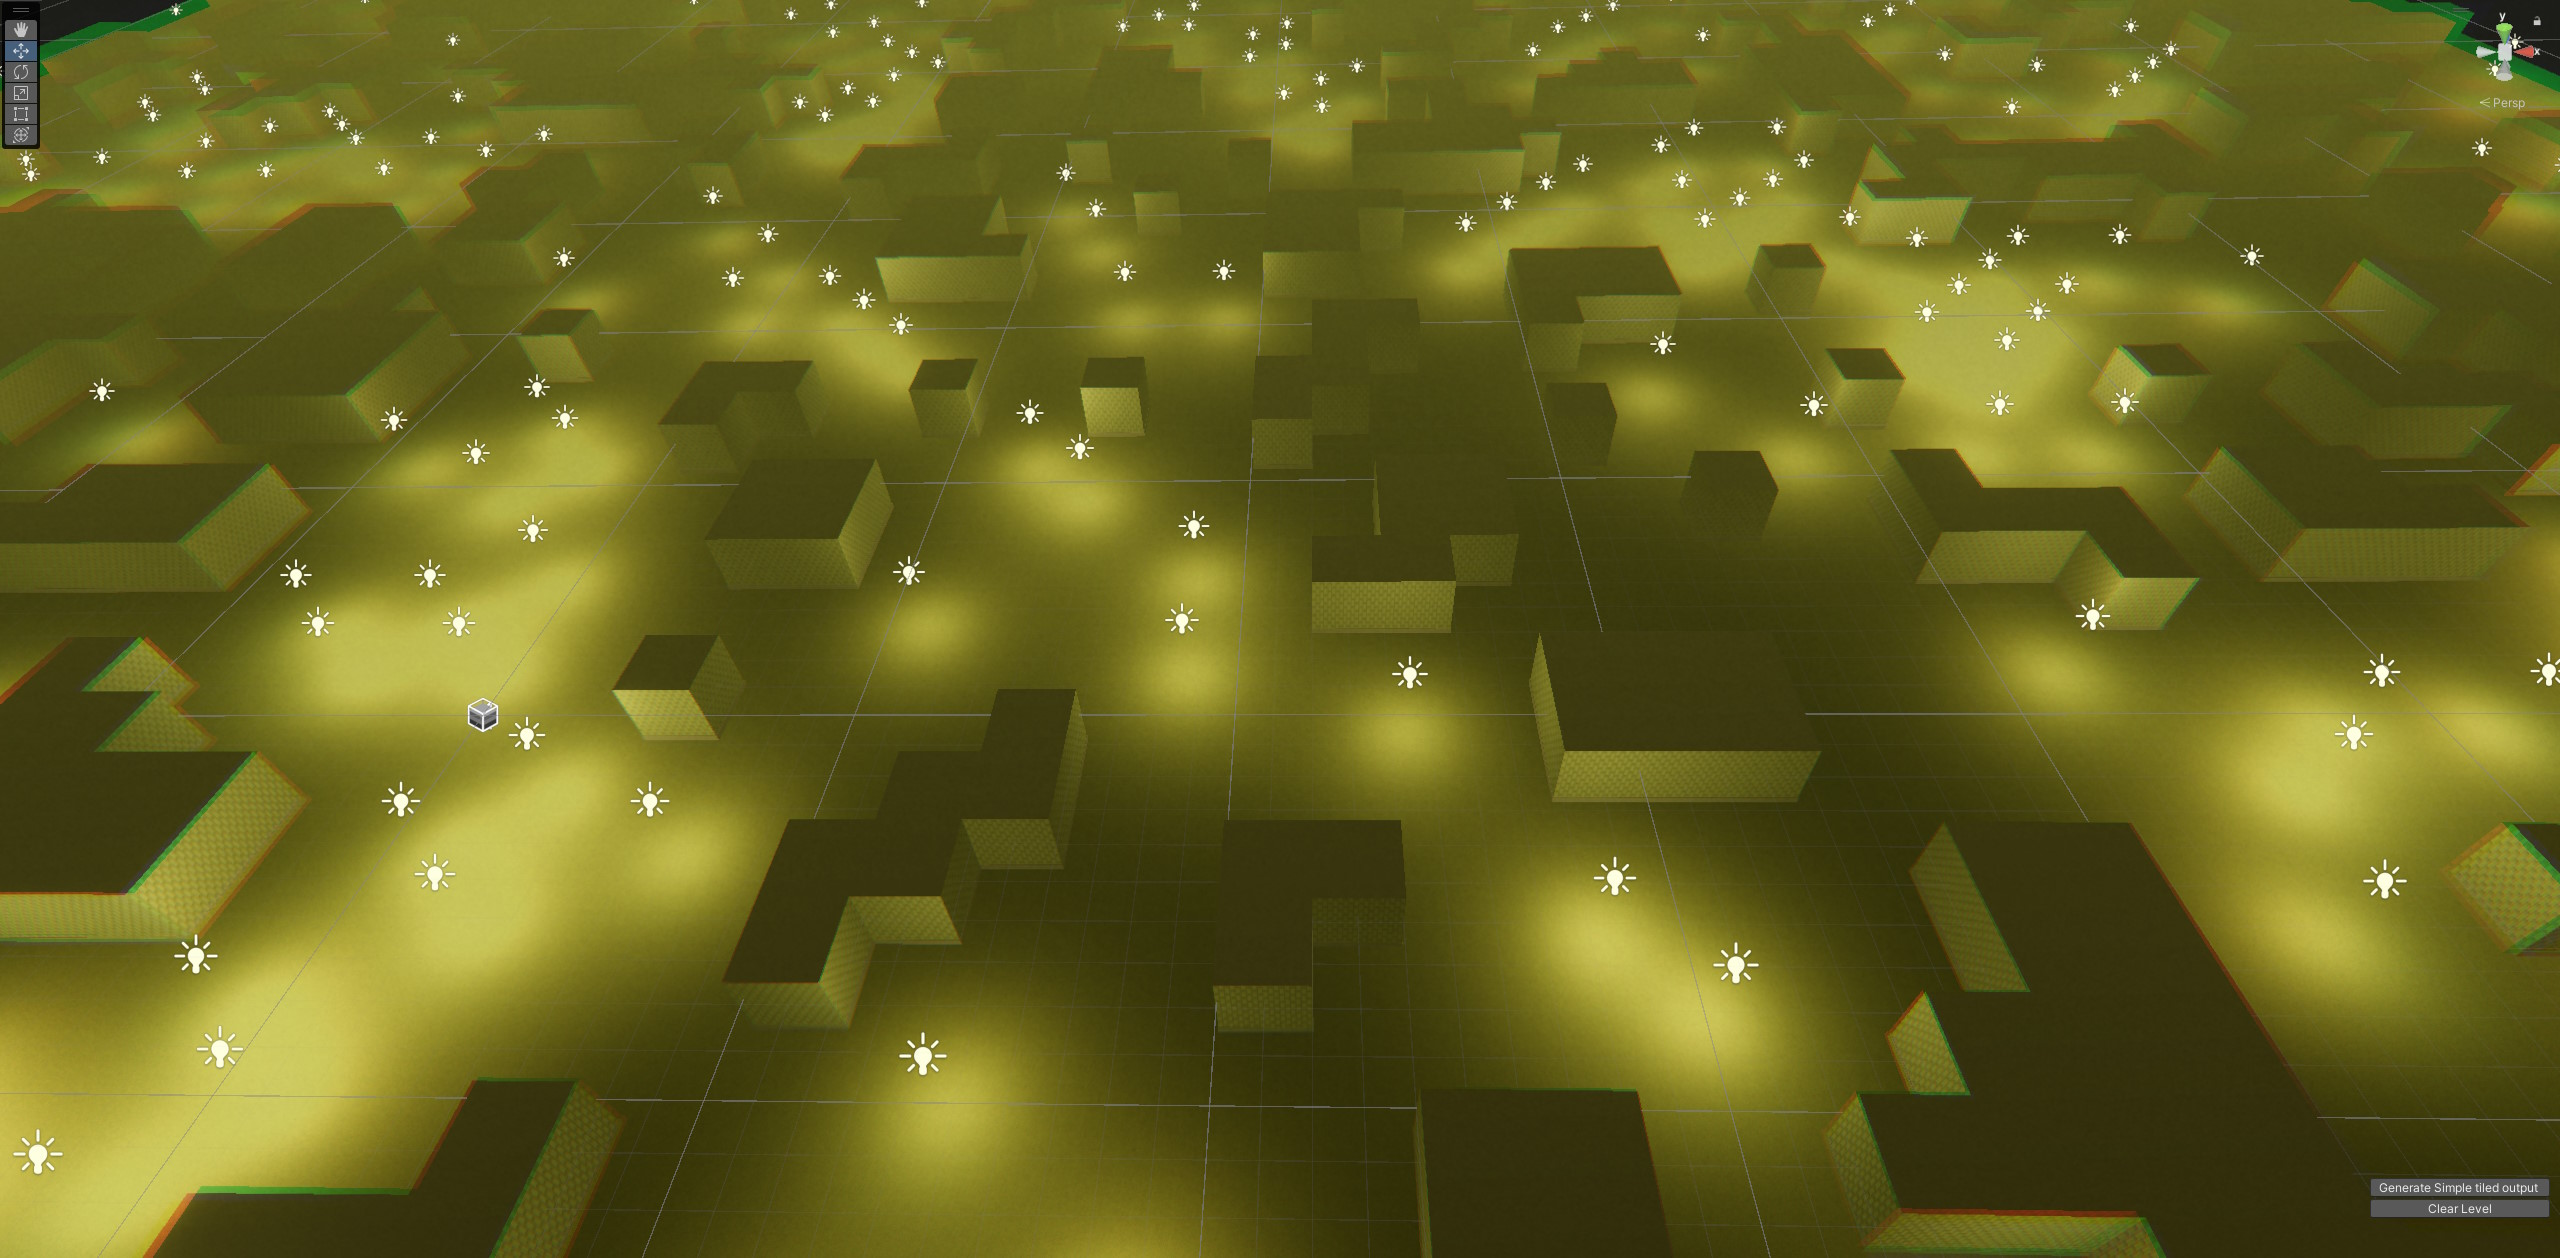
\includegraphics[width=0.475\textwidth, height=0.2\textheight, keepaspectratio]{Images/BackroomsIMIB3.jpg}
        \label{fig:backroomsIMIB3}
    }
    \hfill
    \subfigure[Generation of layer 4]{
        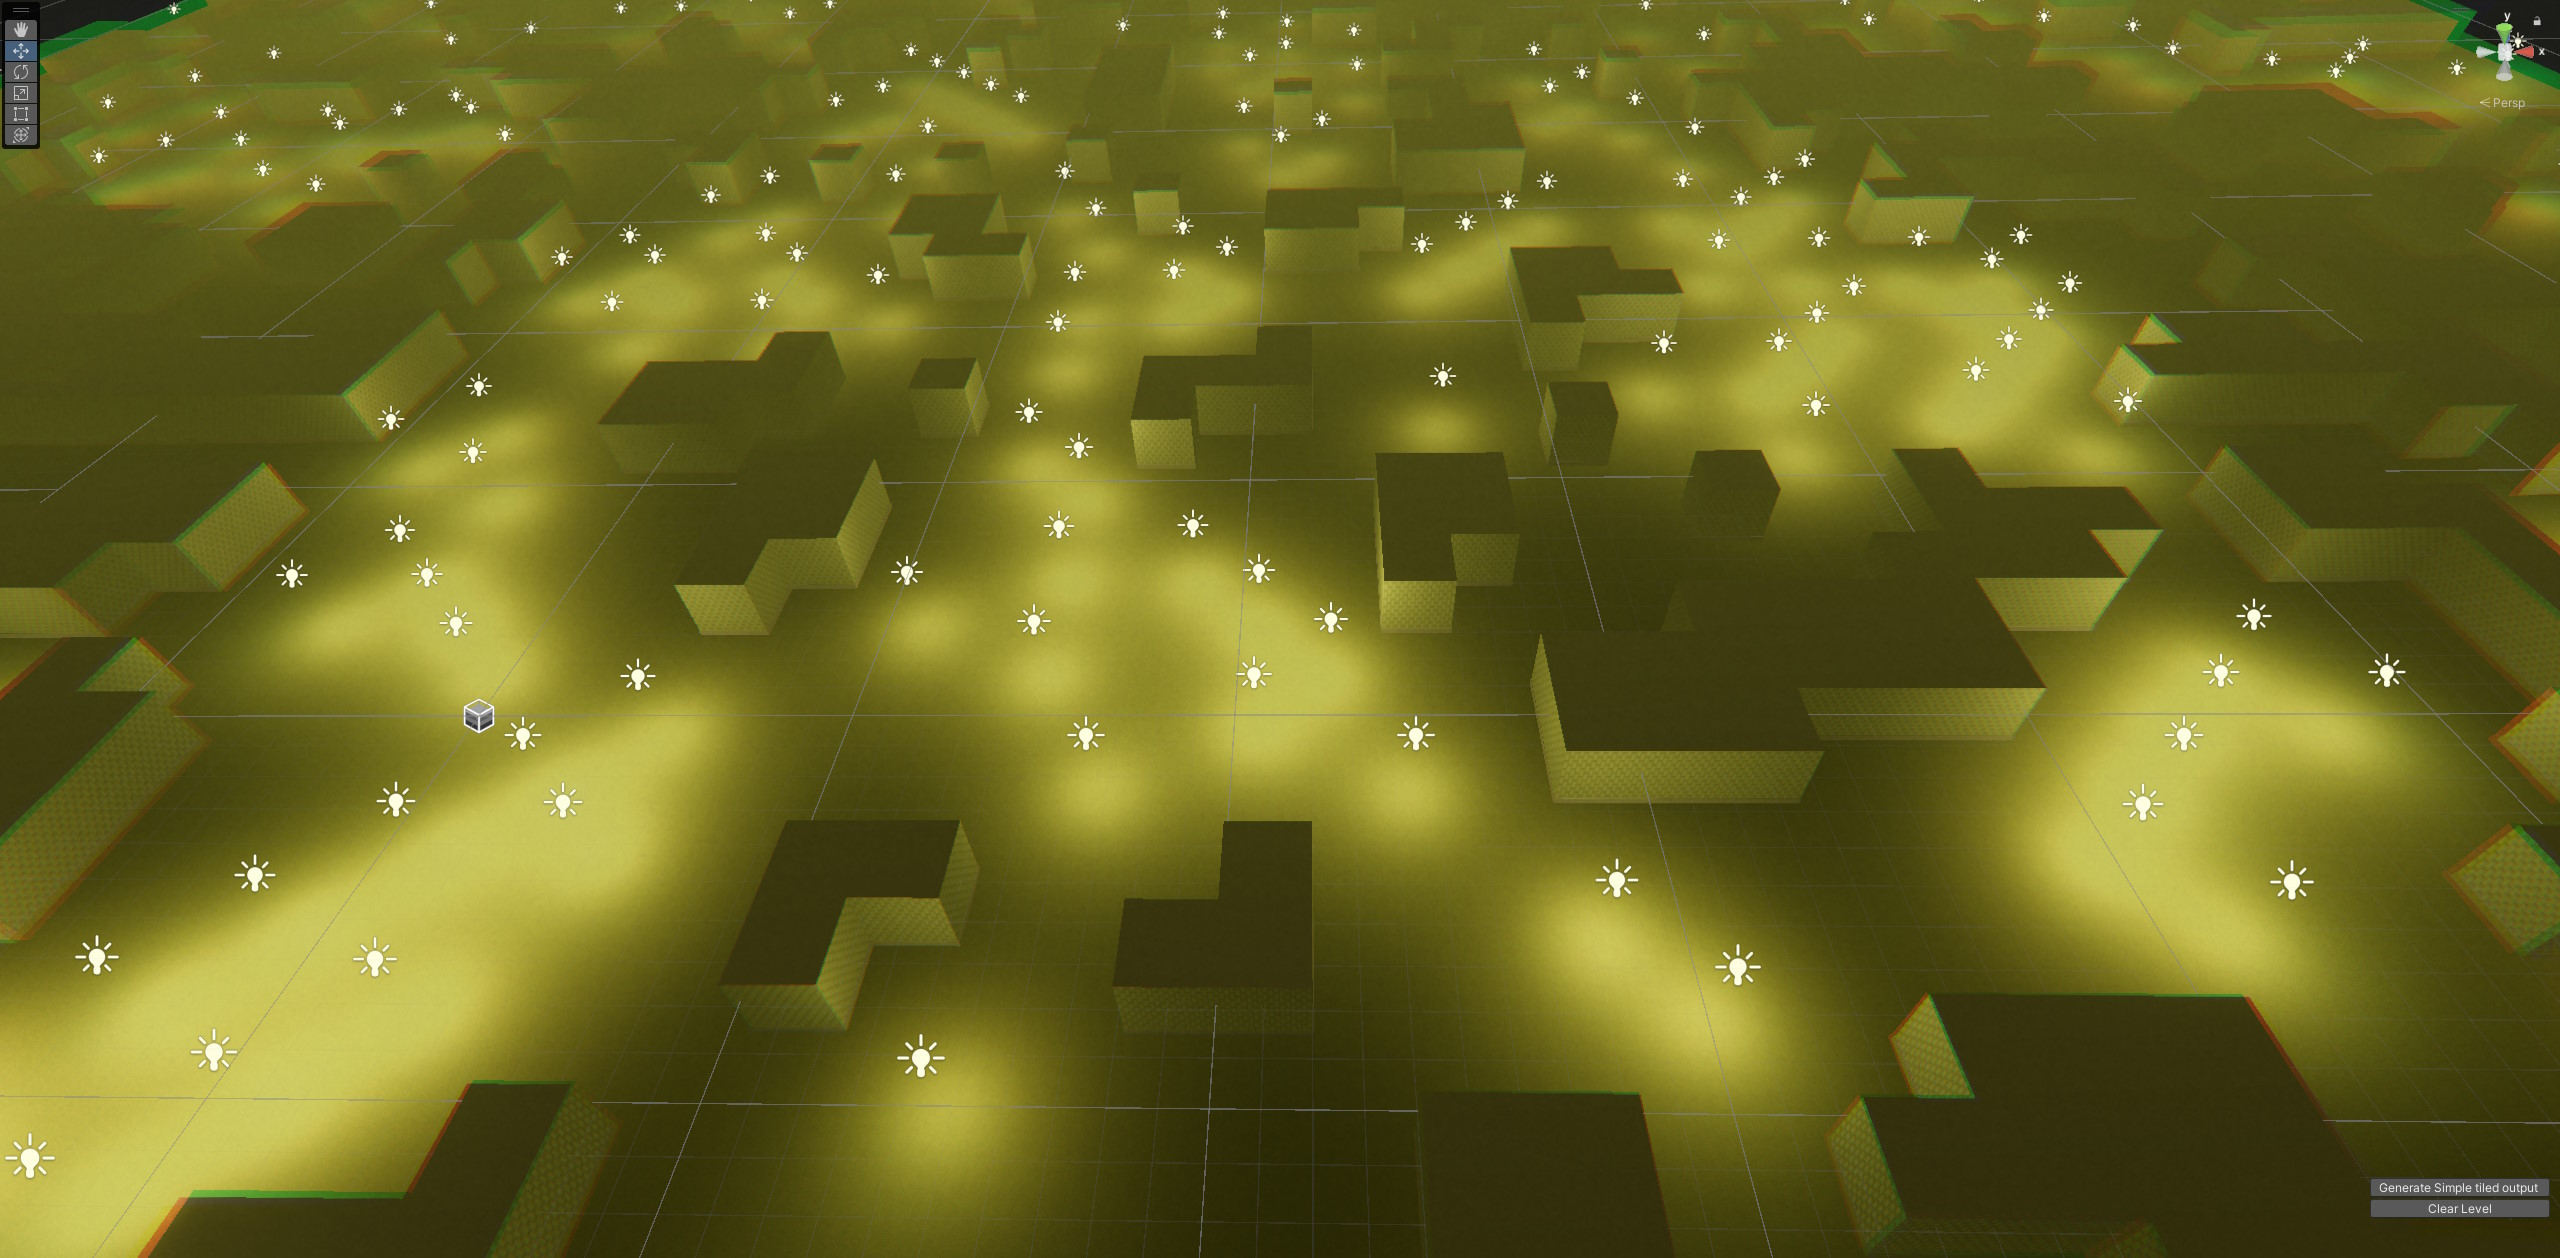
\includegraphics[width=0.475\textwidth, height=0.2\textheight, keepaspectratio]{Images/WeightsNormal.jpg}
        \label{fig:backroomsIMIB4}
    }
    \caption{Running \acrshort{imib} with \textit{the Backrooms} tile set}
    \label{fig:backroomsIMIB}
\end{figure}

Another component to consider is how to load new chunks and unload existing chunks when the player moves about. To do this efficiently, direct calculation of new chunks to load relative to old chunks is performed. As example, Figure \ref{fig:imibMovement1} shows chunks loaded around the player. When the player moves across to another chunk, new chunks must be loaded (blue) and some of the existing chunks unloaded (orange) (Figure \ref{fig:imibMovement2}). By calculating the horizontal and vertical difference in chunk coordinates between the player and the old chunks, the coordinates of the new chunks can be mapped from the old chunks (Figure \ref{fig:imibMovement3}).

% Diagram of 3x3 grid where player moves diagonally.
\begin{figure}[H]
    \centering
    \subfigure[Chunks loaded before the player moves]{
        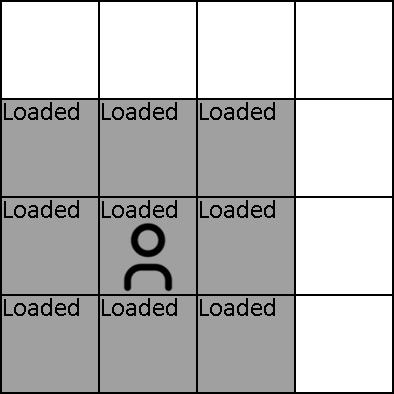
\includegraphics[width=0.3\textwidth, height=0.3\textheight, keepaspectratio]{Images/IMIBMovementBefore.png}
        \label{fig:imibMovement1}
    }
    \hfill
    \subfigure[Chunks after the player moves. Existing chunks are shown in grey, chunks to unload in orange and chunks to load in blue.]{
        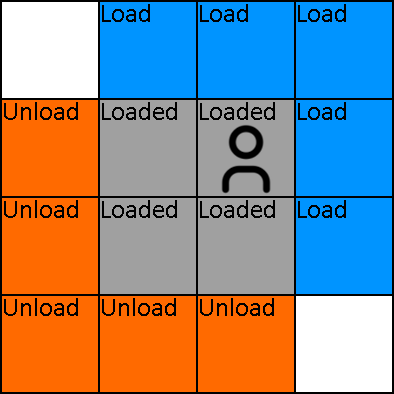
\includegraphics[width=0.3\textwidth, height=0.3\textheight, keepaspectratio]{Images/IMIBMovementAfter.png}
        \label{fig:imibMovement2}
    }
    \hfill
    \subfigure[Arrows showing how chunks are mapped to each other]{
        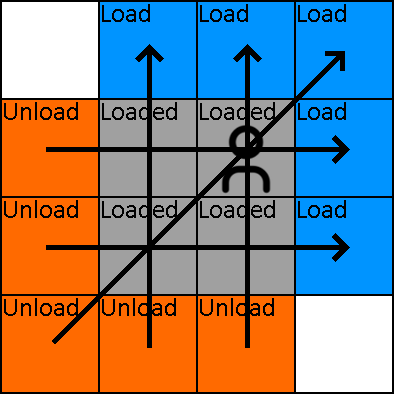
\includegraphics[width=0.3\textwidth, height=0.3\textheight, keepaspectratio]{Images/IMIBMovementAfterWithArrows.png}
        \label{fig:imibMovement3}
    }
    \caption{The chunks to unload and load in an infinite world can be mapped directly from their relative position to the player}
    \label{fig:imibMovement}
\end{figure}

\section{Unity Editor and Tile Representation}
The Unity Editor was used to provide a platform with which level designer could specify parameters for level generation. First, the level designer should attach the Level Generation Manager component to a unity game object. The designer may specify the size of chunks use in \acrlong{imib}. Tiles are split into three different components across the entire specification to generation pipeline, with the tile set for generation specified in steps 1 and 2.
\begin{enumerate}
    \item The level designer must first specify tiles by creating Unity game objects and then attaching a subclass of the Tile component to it. The Cube subclass exists for fully-symmetric tiles and the NonSymmetric subclass exists for all other tiles. The designer can then specify tile adjacencies by dragging other tile game objects into the neighbours arrays and specifying the desired rotation of the neighbouring tile. Base rotations of tiles should have their solid face at the back of the tile. The base rotation for corner tiles has the back of the corner on the left and back of the tile. Each game object should then be dragged into the tile set array of the level generator. Additionally, an empty tile must be specified directly.
    \item After specifying tile adjacencies, the level designer should import FBX models to form a second set of game objects. These should be given a collider to avoid the player falling through the level. The designer can also add any additional components such as lights or audio sources. These model game objects can then be referenced in the matching tile script component. This tells the level generator to use the desired model for a given tile. The tile size specified in the level generator must match the size of the tile models in order for the generator to put them together properly.
    \item Finally, the tile set that the level designer specified is converted from the designer-specified semi-explicit tile set to a fully-explicit tile set. The level generator takes each specified tile and rotates it in steps of 90 degrees, adjusting adjacency data to suit. This gives each possible rotation of a tile its own tile, hence the term fully-explicit. In effect, this enables the generation of maps without having to perform intermediate calculations on tile rotation, simplifying the algorithm at the cost of a larger tile set.
\end{enumerate}

% Diagram of specification to generation pipeline. Define cardinality / rotation clearly in the diagram. Maybe also in text more clearly or somewhere else.

\section{Game Design}
The premise of the game was inspired by the fictional concept of \textit{the Backrooms}. These encompass an endless collection of `levels', each a potentially infinite space with a unique theme centred around invoking a feeling of liminality. This was deemed a suitable theme to use for a game exploring novel \acrlong{pcg} techniques. The first level of \textit{the Backrooms}, `Level Zero', resembles an empty office-like space. Yellow wallpaper, light brown carpet and bright fluorescent lights combine to give it an unsettling monotone appearance and soundscape. The player controller was taken from an online tutorial \cite{FPS_controller_YouTube, FPS_controller_GitHub}. This allows the player to move around the level.

% Side-by-side Image of the backrooms with image in-game

%Additionally, the ability to pick up and drop items was added. This allows the player to solve puzzles throughout the world.
%\subsubsection{Puzzles}
%The player must explore the Backrooms in search of items spawned randomly with the level geometry.
% REMEMBER: COLLECT ITEMS TO REPAIR SOMETHING!
% Goal walls are locked doors. Adjacent to them are fuse boxes?
% Old idea (?):
% Goal walls are locked doors. Safe in wall containing key. Safe requires finding combination / power out?
%\begin{enumerate}
%\item Find 
%\end{enumerate}

\section{Graphics}
\subsection{Models and Textures}
The models with texturing for each tile were made in the software Blender using a YouTube video as a guide \cite{backroomsGraphics}. The tiles have distinct shapes, but share common wallpaper \cite{sketchfab_texture}, ceiling tile \cite{ceiling_texture} and carpet textures \cite{carpet_texture}. These textures are mapped so that they appear continuous when tiles are placed next to each other. The carpet texture does not connect seamlessy when rotated, so a workaround is used. This spawns the floor separately for each tile, ensuring each carpet piece has the same orientation. Each of the models used is shown in Figure \ref{fig:blenderTileSet}. From left to right, the models include a cube, corner, corner pillar, wall, centre pillar and empty tile.

% Image of tiles in Blender. Write text to define each.
\begin{figure}[H]
    \centering
    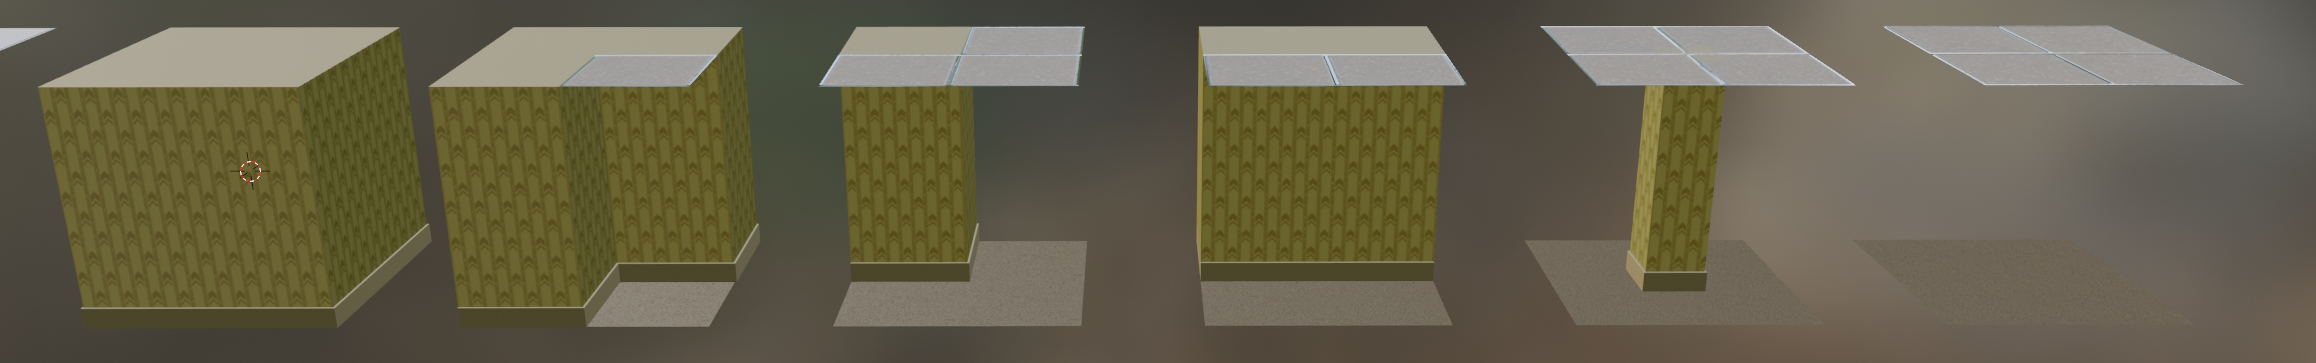
\includegraphics[width=\textwidth, height=0.3\textheight, keepaspectratio]{Images/Tileset.jpg}
    \caption{The model tile set in Blender}
    \label{fig:blenderTileSet}
\end{figure}

\subsection{Visual Effects}
Unity's Universal Render Pipeline was used to give additional control over rendering and visual effects. To simulate the appearance of a video recorded onto a VHS tape, a range of camera effects were used. These are listed in Figure \ref{fig:cameraEffects}. Furthermore, the player's camera is rendered to a render texture with a resolution of 640 by 480 \cite{vhsGraphicsGuide} and a letterbox used \cite{letterboxer_github}, further enhancing the image.

\begin{figure}[H]
    \begin{framed}
        \begin{itemize}
            \item Depth of Field: Blurs objects that are very close to the camera, simulating depth.
            \item Bloom: Increases the effect of light on the scene, emulating high sensitivity. Also includes a lens dirt texture \cite{actionvfx_lens_dirt}.
            \item Motion Blur: Simulates unclear image capture from moving the camera.
            \item Tonemapping (ACES): Maps colour tones differently to give a filmic effect, making the image appear more realistic.
            \item Lens Distortion: Shifts projection around the centre of the image to simulate capture through a lens.
            \item Film Grain: Adds noise to the image to simulate similar noise real cameras can capture.
            \item Chromatic Aberration: Disperses red, green and blue colours at the edge of the screen to simulate the same effect lenses can exhibit in real life.
            \item Panini Projection: Shifts projection to better render perspective views in wide angle scenes. Acts as additional distortion to make the image appear more organic.
            \item Color Adjustments: Reduces exposure to make tones more neutral. Also adds a colour filter to shift colours slightly more towards monochrome yellow to fit the level theme.
            \item Fog: Obscures distant objects to hide the border of currently generated chunks.
            \item VHS Overlay Videos: Adds additional noise seen when playing VHS tapes \cite{vhsGraphicsGuide, enchanted_media, youtube_video3}.
        \end{itemize}
    \end{framed}
    \caption{Camera Effects}
    \label{fig:cameraEffects}
\end{figure}

\subsection{Lighting Model}
A deferred lighting model was used to light the level \cite{lighting_models}. Unity's default lighting relies heavily on baked lighting to provide for high quality lighting. Baking lighting describes pre-calculating lighting before runtime. Textures can then be illuminated cheaply at runtime using this baking data to help give levels a realistic look. As the project uses procedurally generated levels, it must heavily rely on realtime lighting instead. This describes lighting that is calculated at runtime as opposed to baked lighting. However, forward rendering (Unity's default rendering method) only allows for a limited number of realtime light sources to be rendered at once. Deferred lighting instead supports many realtime lights at the cost of less accurate lighting. Figure \ref{fig:renderingModels} compares forward and deferred rendering in a generated level, showing that deferred is more suited to rendering many light sources.

% Compare two images. One is forward rendering of a generated level and the other deferred.
\begin{figure}[H]
    \centering
    \subfigure[Forward rendering fails to compute lighting accurately with many light sources]{
        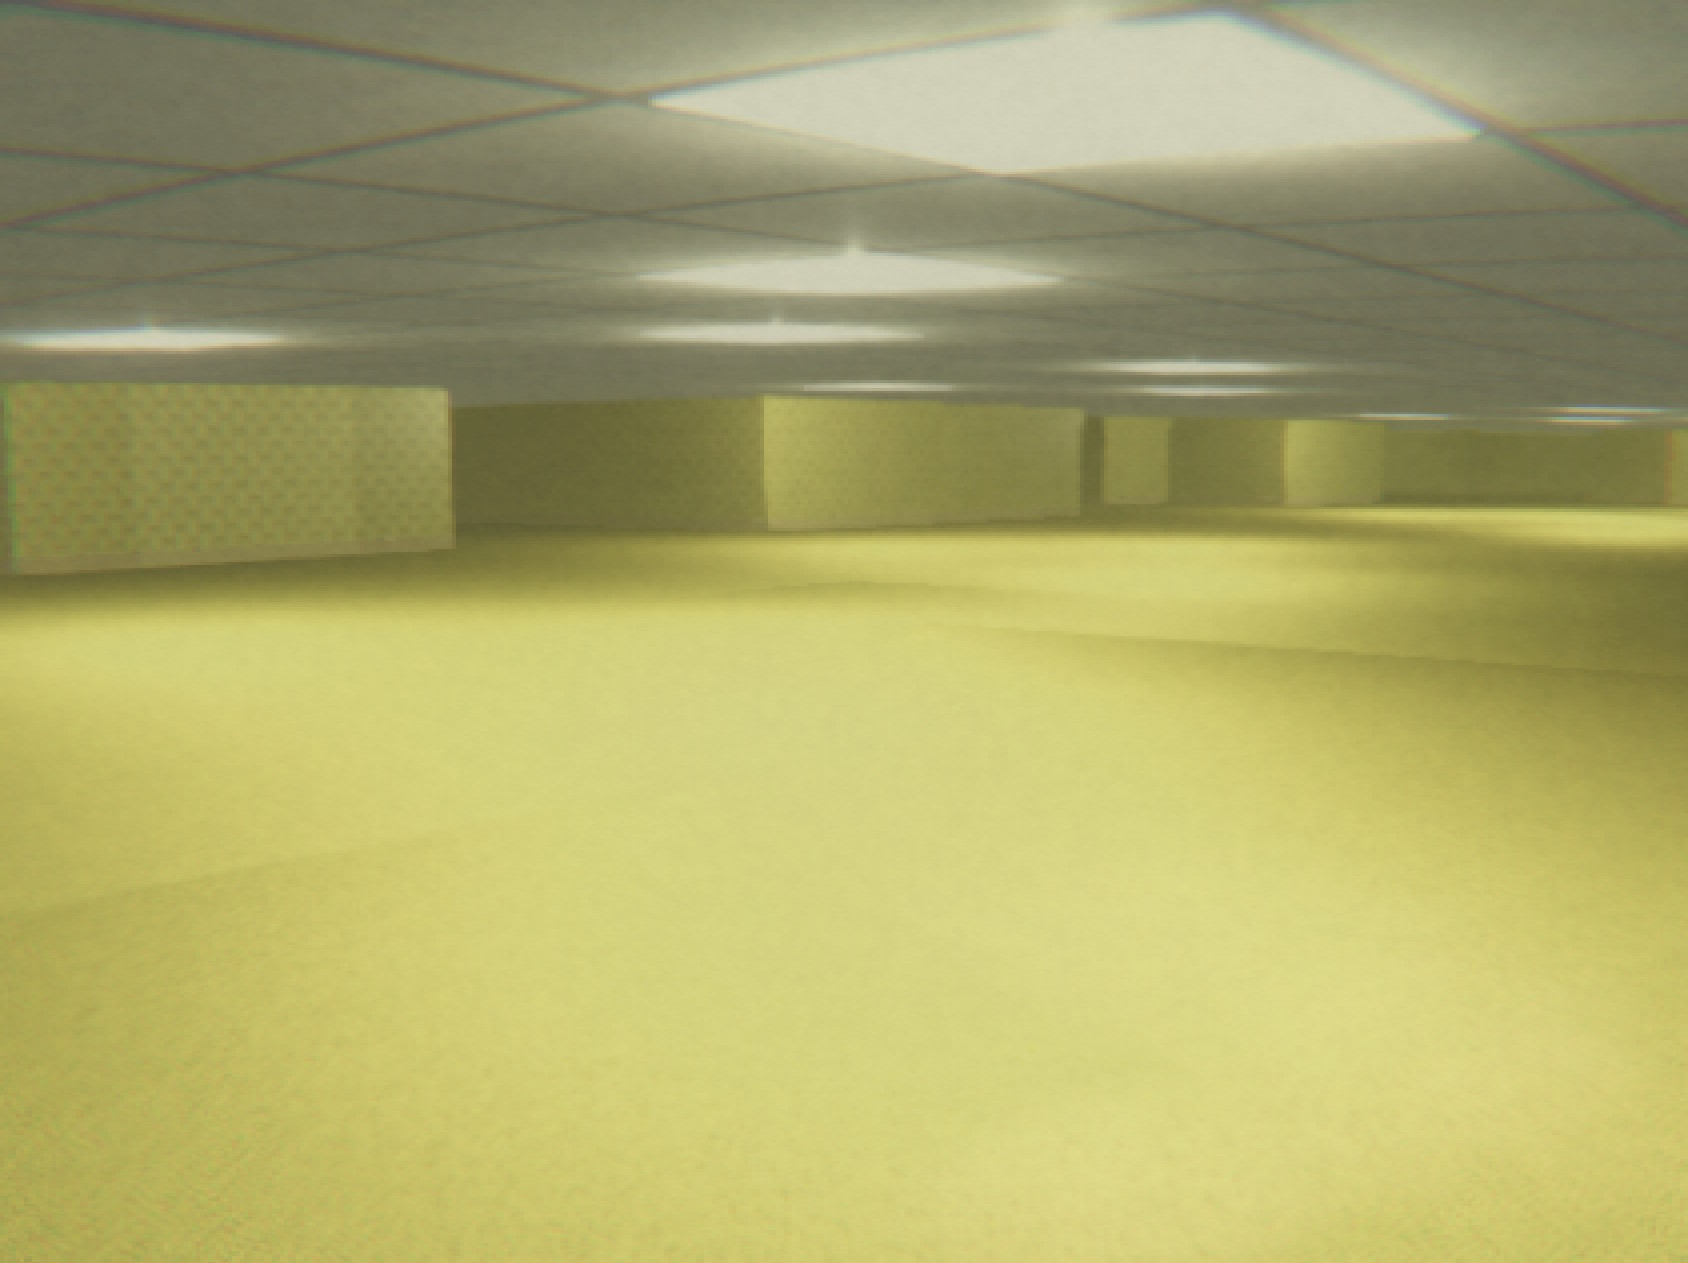
\includegraphics[width=0.475\textwidth, height=0.3\textheight, keepaspectratio]{Images/RenderingForward.jpg}
        \label{fig:renderingModels1}
    }
    \hfill
    \subfigure[Deferred lighting is more suited to many light sources]{
        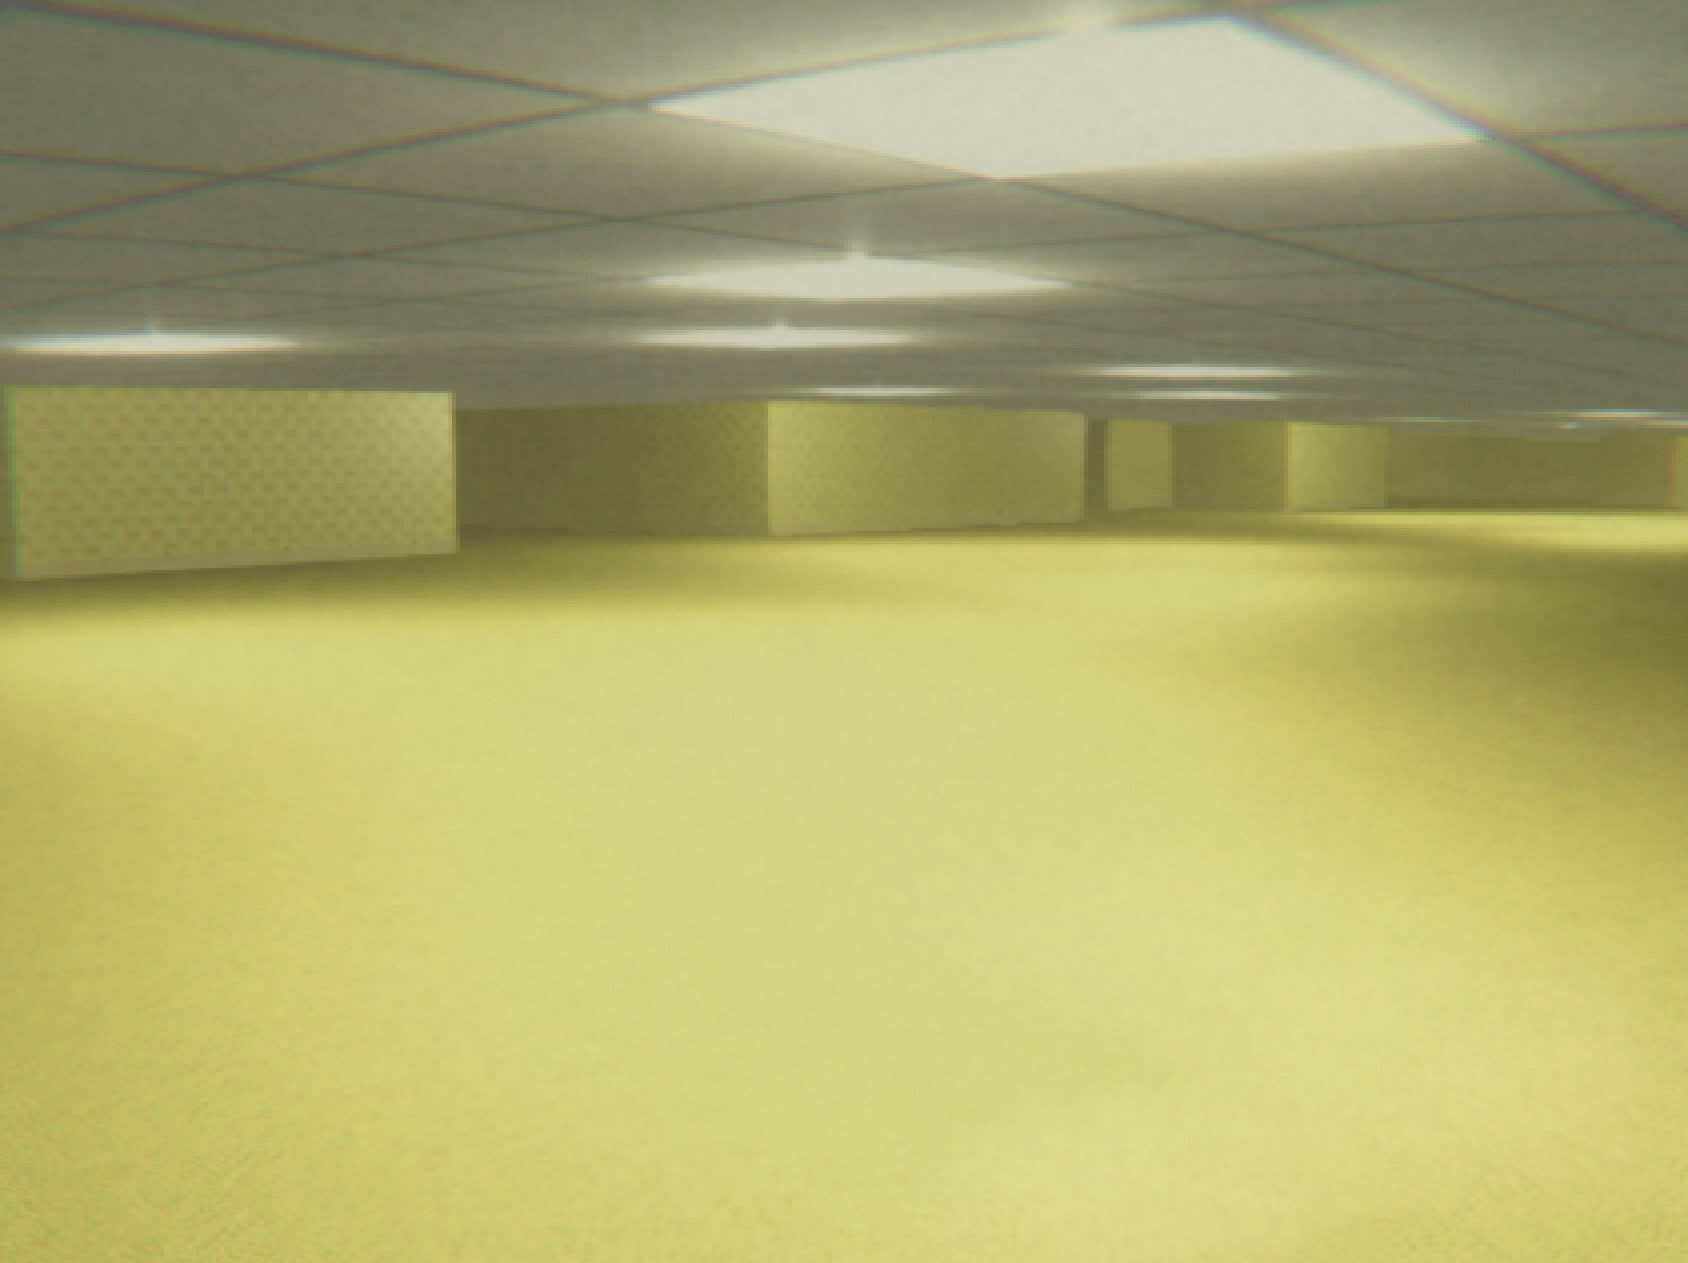
\includegraphics[width=0.475\textwidth, height=0.3\textheight, keepaspectratio]{Images/RenderingDeferred.jpg}
        \label{fig:renderingModels2}
    }
    \caption{A comparison of forward and deferred lighting. Forward lighting fails to light the scene properly, showing distinct lines on tiles.}
    \label{fig:renderingModels}
\end{figure}

\section{Audio}
To give the game area an immersive soundscape, a collection of ambient effects and sound effects were used. Ambient effects are those sounds that are played equally at all times, while sound effects are those sounds that are placed inside of the environment. The most distinct sound effect of Level Zero of the Backrooms is the buzzing of the fluorescent lights. Each empty tile with a light is given an audio source that plays such a sound \cite{fluorescent_sound}. Each light is given its own random offset so that the audio does not poorly overlap and cause constructive interference. For ambient sounds, a VHS sound is included \cite{vhs_sound}. All audio assets were taken from \url{freesound.org} as this site offers sounds free for use in games.